\chapter{Performance Analyse relationaler Lösungswege}

Um die Performance der im zweiten Kapitel beschriebenen Lösungswege zu testen, wurde ein Programm geschrieben. Zunächst wird beschreiben, auf welche Parameter die verschiedenen Lösungswege untersucht wurden. Anschließend betrachten wir den Testaufbau, d.h. die verwendeten Technologien und die Struktur des Testprogramms. Dabei wird auf mehrere Probleme bei der Umsetzung und auf Lösungen für oder Einschränkungen durch diese eingegangen. Am Ende des Kapitels werden die Laufzeiten verglichen und Aussagen zu den Ergebnissen getroffen.

\section{Test-Dimensionen}

Um die Effizienz unserer Lösungswege zu bestimmen, müssen mehrere Aspekte untersucht werden. Da jeder dieser Aspekte die Anzahl an Testergebnissen multiplikativ erhöht, werden sie Test-Dimensionen genannt.

Die erste Dimension ist die Anzahl der Elemente in der Datenbank. Durch die Untersuchung mit unterschiedlicher Anzahl von Elementen in der Datenbank lassen sich Aussagen über die Skalierbarkeit der Lösungsansätze treffen. Für die konkreten Tests wurde beschlossen, die Fälle mit jeweils 100.000 und 1.000.000 Elementen in der Datenbank zu untersuchen.


\subsection{Wahl der Datenbank}
\label{ssec:database}

Um eine starke Lösung zu finden müssen nicht nur unterschiedliche Ansätze, sondern auch die jeweiligen Datenbanken, in denen die Ansätze durchgeführt werden, gezielt ausgewählt werden. Um Vergleichbarkeit zu schaffen sollten die Datenbanken sowohl für den Einsatz von EAV als auch der JSON Methode geeignet sein. Hier ist eher die Unterstützung von JSON Elementen interessant, da der EAV Ansatz keine besonderen Voraussetzungen besitzt. Die Auswahl kann via dem Kriterium, ob eine Datenbank Indizies für den JSON Datentyp bereitstellt, eingegrenzt werden.

%Ein weiterer Betrachtungspunkt ist, wie stark etabliert eine Datenbank ist. 

% technology adoptation life cycle -> einschätzung eigenes profil??

Nach Betrachtung der beschriebenen Anforderungen wurden zwei Datenbanken gewählt.

Die erste Wahl fiel auf PostgreSQL. PostgreSQL ist eine freie Open-Source-Datenbank. Die verwendete Version war die zum Zeitpunkt des Beginns der Entwicklung aktuellste Version, 13.1 (Debian 13.1-1.pgdg100+1). PostgreSQL qualifizierte sich durch extra Datentypen für JSON Elemente und eines speziellen Index für diese Datentypen. Zusätzlich erweitert PostgreSQL die SQL Syntax mit speziellen Befehlen, die für die Verarbeitung von JSON Elementen erstellt wurden.

%Befehle 
Um JSON Elemte in der Datenbank abzulegen, existieren zwei Datentypen: \lstinline|json| und \lstinline|jsonb|. \lstinline|json| legt den übergebenen Wert direkt in der Datenbank ab, während \lstinline|jsonb| den Wert in ein Binärformat umwandelt. Das  erleichtert den Umgang mit den gespeicherten Daten, vor allem da dadurch der Einsatz von Indizes ermöglicht wird. Daher wurde in der Testanwendung auch der Typ \lstinline|jsonb| verwendet.


Für die beiden JSON-Querys wurde folgender Befehl verwendet:
\begin{lstlisting}[language=SQL, caption={PostgreSQL Querys}]
SELECT * FROM pages WHERE attributes::jsonb @> ?::jsonb
\end{lstlisting}
Das Fragezeichen steht als Platzhalter für einen Parameter, der unseren Suchtext beinhaltet. Der Operator \lstinline|@>| ist ein Containment Operator. Er überprüft, ob das erste Element das Zweite beinhaltet. Das Element, das für die Suche in die Query eingefügt wird, wurde per Hilfsmethode aus den gesuchten Parametern erstellt.  \cite{PostgreSQLDocumentation.2021}

Die zweite Datenbank, die untersucht wird, ist Oracle Database. Im speziellen Oracle Database Express Edition (Oracle Database XE) 18c. Die Lizensierung der Oracle Database erschwert es, das neuste Release, zur Zeit der Veröffentlichung dieser Arbeit 21c, der Datenbank zu testen. Oracle stellt regelmäßig bestimmte Versionen, deren Lizenz nicht käuflich erworben werden muss, frei zur Verfügung. Diese Releases werden Express Edition genannt. 

Eine Einschränkung dieser Version ist eine geringe maximale Speichergröße von 12 GB. Diese Begrenzung mach es unmöglich, den Test mit 1,000,000 Einträgen durchzuführen, sowohl mit dem EAV als auch mit dem JSON Ansatz. Daher konnte in der Oracle Umgebung nur die kleineren Tests mit weniger Testdaten durchgeführt werden. \cite{oraclexe.13.07.2021}

Oracle Database bietet einen Check für die JSON-Konformität für Spalten und spezielle SQL Syntax für die Abfrage von JSON Elementen. Zusätzlich können Indizes basierend auf bestimmten Funktionen oder für Volltextsuche für JSON optimiert angelegt werden.  \cite{OracleHelpCenter.2019}

Um eine Spalte als JSON-Spalte zu verwenden, muss ein Constraint verwendet werden. Der Befehl hierzu lautet:
\begin{lstlisting}[language=SQL,caption={Oracle Database JSON Constraint}]
CONSTRAINT "ENSURE_JSON_ATTRIBUTE" CHECK (attributes IS JSON)
\end{lstlisting}
Der Typ der Spalte attributes, der verwendet wurde, ist clob.

Die Syntax für JSON Querys ist anders als bei PostgreSQL. Anstelle eines neuen Operators werden komplette Funktionen verwendet. Operatoren sind jedoch nur syntaktischer Zucker und sollte nicht als wichtiges Argument für oder gegen eine Lösung stehen. Schwerwiegender ist jedoch, dass die Funktionen den Einsatz von Prepared Statements erschweren (vgl. \ref{ppar:JDBC} JDBC). Die Befehle zur Suche von Elementen mit einem bestimmten Attribut und einem bestimmten Attributwert haben den Aufbau 
\begin{lstlisting}[language=SQL,caption={Oracle Database, FindByAttribute-Query}]
SELECT * FROM pages WHERE json_exists(attributes, '$[*]?(@.name == "attributeName")')
\end{lstlisting}
 respektive 
 \begin{lstlisting}[language=SQL,caption={Oracle Database, FindByValue-Query}]
SELECT * FROM pages WHERE json_exists(attributes, '$[*]?(@.name == "attributeName" && @.values[*].value.Type == "value.Value")'
\end{lstlisting}

Der Suchtext liest sich in etwa: Existiert ein Element in einem Array (\lstinline|$[*]|), welches einen Schlüssel mit dem Namen ``name'' und dem gesuchten Attributnamen als Wert enthält (\lstinline|?(@.name == "attributeName")|); und zusätzlich bei der Suche nach einem bestimmten Attributwert ein Array mit der gewünschten Typ-Wert als Schlüssel-Wert Kombination enthält (\lstinline|&& @.values[*].valueType == "valueValue"|).
 
Die Indizes der beiden Datenbanken werden in Abschnitt \ref{ssec:indexes} näher beschrieben.

Zu den ausgeschlossenen Datenbanken zählt u.a. MySQL, welches zwar einen JSON Datentyp und Funktionen für Querys bereitstellt \cite{.10.07.2021}, aber keine Möglichkeit bietet, JSON Felder direkt zu indizieren. Stattdessen wird empfohlen, Indizes auf generierten Spalten zu erstellen \cite{.10.07.2021b}. Dies bezieht sich aber auf feste Schlüssel und keine Array-Werte.


%ein fall große datenbank
\subsection{Anwendungsfälle}

Die nächste Dimension der Testfälle sind die untersuchten Anwendungsfälle. Diese basieren auf den grundlegenden Operationen in der Persistenzschicht von Anwendungen: Create, Read, Update und Delete, oft unter dem Akronym CRUD zusammengefasst. Daraus lassen sich folgende Anwendungsfälle ableiten:

\begin{itemize}
\item Create: Erstellen eines neuen Elements ohne Attribute
\item Read: Abfragen nach Elementen mit bestimmten Attributen und nach Elementen mit bestimmten Attributwerten\footnote{Für die Simulation einer Webanwendung und zur Minimierung der Testlaufzeiten wurde entschieden, dass in Queries eine maximale Fetch-Größe von 100 Einträgen gesetzt ist. Dieses Vorgehen entspricht einer Seiten-basierter Ansicht, bei der weitere Ergebnisse erst nach Aufruf geladen werden. In den Tests wurde jeweils nur die ersten 100 Ergebnisse von der Datenbank aufgerufen. Hier war zu beachten, das die Fetch-Größe explizit gesetzt werden muss und bei PostgreSQL die Verbindung nicht auf Auto-Commit stehen darf. Außerdem kann bei besonders vielen Treffern ohne eine Fetch-Size eine Query bei einer PostgreSQL Datenbank zu einem OutOfMemory Fehler führen.}
\item Update: Änderung eines einzelnen Attributwert
\item Delete: Löschen eines kompletten Elements inklusive aller Attributwerte
\end{itemize}

Zusätzlich wurde ein Testfall mit einem äußert großem Attributwert untersucht. Für Testzwecke wurde der extreme Fall, einen 2 Megabyte(MB) großen String als ein Attribut zu speichern und anschließend weiteren Text anzuhängen, gewählt. Gemessen wurde die benötigte Zeit, um eine Änderung an diesem Text durchzuführen. Dieser Testfall war durch bekannte Problemfälle in existierenden Anwendungen motiviert, führte jedoch zu einer Einschränkung der Testergebnisse. Durch die Notwendigkeit, ein sehr großes Element speichern zu können, mussten teilweise die Datentypen angepasst werden. Dies hatte auch zur Folge, das in der Oracle Umgebung mit dem Ansatz EAV keine Tests mit Indizes durchgeführt werden konnten. Das gleiche gilt für den EAV-Ansatz in PostgreSQL, der mit Indizes nur einen Teil der Anwendungsfälle durchführen konnte. Die restlichen Fälle konnten hier untersucht werden, indem der Fall mit dem großen Attributwert übersprungen wurde (vgl. Absatz \ref{ssec:indexes}).

Die zugehörigen Bezeichnungen für diese Anwendungsfälle in der Auswertung lauten:

\begin{itemize}
\item Create: ``CreatePage''
\item Read: ``FindByAttribute'': Suche nach Elementen, die ein Attribut mit diesem Namen haben\\
``FindByValue'': Suche nach Elementen, die ein Attribut mit einem bestimmten Namen und Wert haben
\item Update: ``UpdatePage''
\item Delete: ``DeletePage''
\item Änderung eines großen Attributs: ``ChangeBigAttribute''
\end{itemize}

% Timings EAV

%mehrere use cases (basis crud)
%zusätzlich anforderung große attribute
\label{ssec:indexes}
\subsection{Indizierung}

Wie bereits beschrieben bieten verschiedene Datenbanken unterschiedliche Indizes an. Um die Wirksamkeit dieser Indizes zu überprüfen wurden die Messungen jeweils einmal mit und einmal ohne spezielle Indizes durchgeführt. Ohne Index heißt in diesem Fall nur mit einem Index auf den jeweiligen Primärschlüssel, der immer und automatisch existiert.
Das ist die vierte und letzte Dimension unserer Tests.

\paragraph{Oracle}

Für das Indizieren von JSON Daten unterscheidet die Oracle Dokumentation zwischen zwei Fällen: Indizierung von festen Attributen innerhalb fester JSON Strukturen, ein Format das dem Standardfall ähnlich den von normalen Spalten entspricht, und einem JSON search index. Da in Rahmen dieser Arbeit beliebig neue Attribute in der JSON Struktur abgelegt werden müssen, ist der JSON search index die erste Wahl. Oracle empfiehlt diesen Index für ad-hoc Queries und full-text search.

% Bei erstem index pro attribut -> sehr groß sehr schnell + dynamische Änderung zur laufzeit
% -> vermutung 2. besser
Um den Ersten, den Value Index, zu verwenden muss zum Zeitpunkt der Erstellung des Index bereits das zu suchende Attribut bekannt sein. Daher müssten wir, um diesen Index zu verwenden, für jedes neue Attribut zur Laufzeit einen neuen Index anlegen. Das kann je nach Art der verwalteten Daten zu großen Perfomance-Problemen führen, da die Anzahl an Indizes zusammen mit der Zahl der Attributen im System steigt. Dadurch könnte die Leistung bei Create und Update Operationen leiden, falls die Indizes sofort die neuen Einträge enthalten müssen. Eine Möglichkeit, diese Gefahr zu umgehen, wäre ein regelmäßiger Job, der die Indizes zu Zeiten aktualisiert, bei denen die Grundlast sehr niedrig ist, etwa während der Nacht.

Der Search Index dagegen kann für beliebige Werte verwendet werden. Er kann genauso wie der Index für feste Werte asynchron verwendet werden. \cite{OracleHelpCenter.2019}

Der EAV Ansatz würde hingegen keine speziellen Indizes benötigen, sondern nur Indizes die weitere Spalten beinhalten. Leider konnten für diesen Ansatz keine Tests mit Indizes durchgeführt werden. Der Testfall ``ChangeBigAttribute'' schränkt den verwendeten Datentyp, der mindestens etwas mehr als 2MB speichern können muss, für Attributwerte stark ein. Um einen möglichst großen Attributwert abspeichern zu können wurde der Datentyp clob verwendet. Dieser kann sehr große Datenmengen enthalten, ist jedoch für die Verwendung von den benötigten Indizes nicht geeignet. Da nicht wie bei PostgreSQL ein Fehler erst bei der Durchführung dieses Anwendungsfalls, sondern bereits bei der Erstellung des Index auftrat, wurden auch die restlichen Anwendungsfälle nicht durchgeführt.



\paragraph{PostgresSQL}

Auch PostgreSQL bieten mehrere Indizes für \ac{JSON} bzw. Volltextsuche an. Empfohlen wird der sogenannte \acf{GIN} \cite{PostgreSQLDocumentation.2021}. Hier handelt es sich um einen Index, der speziell für Werte verwendet werden kann, die aus Teilwerten bestehen. Dazu gehört der verwendete Typ jsonb, aber auch Arrays vieler verschiedener Typen und Typen für Textsuche. Ein \ac{GIN} legt einen Eintrag in dem Index für jedes Teilelement der zu indizierenden Daten an. Die Grundstruktur ähnelt der eines B-tree Index. Auf Blatt Ebene speichert ein \ac{GIN} anstelle der Spaltenwerte der Reihe, die indiziert wird, eine Liste oder einen weiteren binär Baum mit Pointern auf Reihen, die diesen Teilwert besitzen. Dabei ist jede Wert-Pointer Kombination einzigartig. Die Wahl, ob eine Liste oder eine Binärbaum von tids, die der Datentyp für solche Pointer ist,verwendet wird, hängt von der Anzahl an Reihen mit diesen Teilwerten ab. Diese heißen ``posting list'' respektive ``posting tree''. Da das Einfügen neuer Daten in diese Struktur sehr aufwendig ist, existiert eine weitere Liste, genannt ``pending list'', in der neue Einträge zwischengespeichert werden. Erst wenn diese Liste vollläuft werden die Änderungen in den Index verschmolzen. Davor werden bei der Verwendung des Index sowohl der Baum als auch die ``pending list'' durchsucht. \cite{Grandjonc.24.10.2020}

%siehe theorie
%betrachtung ohne index und mit index, je nach fall

%oracle ist indizierung nicht möglich, da großes textfeld(big attribute case) benötigt -> clob -> kein index auf clob...
\label{sec:testaufbau}
\section{Testaufbau}

%Umsetzun der Ansätze in Java (Webanwendungen, Markanteil?)
Um die Performance aller Tests aufzunehmen und vergleichbar zu machen wurde eine Java Anwendung programmiert. Mithilfe einer kompletten Anwendung lassen sich alle Verarbeitungsschritte zusammen messen und komplexe Versuche einfacher aufgestellt werden. 


\subsection{Programmiertechnische Umsetzung}

Auf dem ``Popularity of Programming Language index'' liegt Java zum Zeitpunkt dieser Arbeit auf Platz zwei \cite{pypl.01.07.2021}. Außerdem existieren im Java-Umfeld bereits mehrere Frameworks, die ähnliche Problemstellungen lösen, i.e. Hibernate. Zusätzlich kann Dank \ac{JDBC} Treibern leicht Datenbankverbindungen hergestellt werden. Daher wurde Java als Programmiersprache für die Testanwendung verwendet. 

Das gesamte Programm kann zur genauen Untersuchung unter \url{https://github.com/matthias-epos/dynamic-datamodels} gefunden werden.

\label{ppar:JDBC}
\paragraph{\acf{JDBC}}
\ac{JDBC} und ähnliche Schnittstellen erlauben es, Code allgemein für verschiedene Datenbanken zu schreiben. Dank spezieller Klassen und Interfaces kann die Kopplung an bestimmten Datenbanken minimiert werden. Voraussetzung dazu ist, dass der Datenbankanbieter eine Implementation des JDBC Treibers zur Verfügung stellt. Der Treiber bildet die Brücke zwischen einer Java-Anwendung und eines Datenbankmanagementsystems. Die Interaktion mit dem Treiber wird über die JDBC API gesteuert. Sie liefert Klassen für alle Aspekte, die für die Interaktion benötigt werden. Dazu gehören unter Anderem \lstinline|Datasource|s, die für Datenbankinstanzen stehen und \lstinline|Connection|s, mit denen SQL Statements erstellt und ausgeführt werden können \cite{Reese.2000}. Ein SQL Befehl kann mit passender Konfiguration so ausgeführt werden:

\begin{lstlisting}[caption={Prepared Statement mit JDBC}]
// conn ist ein vorbereitetes Connection Objekt
stLoadPage = conn.prepareStatement("SELECT * FROM pages WHERE id = ?");
stLoadPage.setLong(1, pageId);
	
rsLoadPage = stLoadPage.executeQuery();
\end{lstlisting}

Hier handelt es sich um ein Prepared Statment. Diese Struktur erlaubt es, Parameter auf eine Art in eine Query einzufügen, die SQL-Injection Angriffe unmöglich macht. Angriffe dieser Art entstehen, wenn ein SQL-Befehl mithilfe eines Strings, der zur Laufzeit zusammengebaut wird, erstellt wird. Sie funktionieren, indem der beabsichtigte Befehl mithilfe eines \lstinline|;| Zeichens verfrüht abgeschlossen wird und ein anderer Befehl, der z.B. beliebige Informationen auslesen könnte, mit angehängt wird.

Innerhalb des Texts, mit dem das Prepared Statement erstellt wird, markieren Fragezeichen Stellen, an denen Parameter eingefügt werden müssen. Dies führt bei den JSON Implementationen der Datenbanken zu Problemen. PostgreSQL benutzt das Fragezeichen als Operator. Um den Operator in einem JDBC Prepared Statement zu verwenden, kann das Fragezeichen mit einem zweitem Fragezeichen escaped werden ($??$). Oracle Database hat ein ähnliches Problem mit den JSON-Funktionen, die für die Querys benötigt werden. Hier gibt es jedoch keine Art, das Problem zu umgehen. Stattdessen muss der Text des SQL Statements dynamisch zusammengebaut werden, was die Anwendung verwundbar gegenüber SQL Injection macht, falls keine weitere Validation der Eingabewerte erfolgt \cite{StackOverflow.14.07.2021}.

%About JDBC
\paragraph{Java Architektur}
Die Anwendung besteht aus mehreren Teilen. Modell-Klassen definieren den Grundaufbau unserer Entities und befinden sich im Package model. 

\begin{figure}[h]
\centering
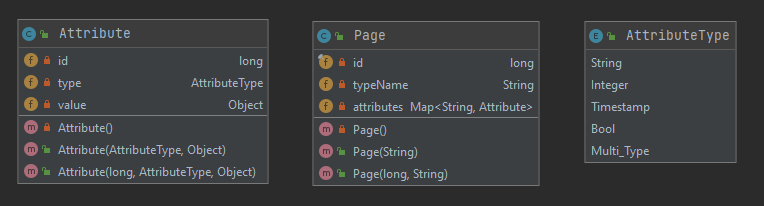
\includegraphics[width=\textwidth]{bilder/model.png}
\caption{Klassenmodell des EAV Ansatzes}
\end{figure}

Die Klasse Page ist die Klasse, deren Objekte mit beliebigen Attributen zur Laufzeit von dem Benutzer erweitert werden kann. Diese Objekte werden in dem Feld attributes, eine <String, Attribute> Map hinterlegt. Ansonsten besitzt sie nur einen Typ-Namen und eine Id. Beim Erstellen eines neuen Page Objekts wird der Wert der Id auf -1 gesetzt. Die echte Id wird erst von der Datenbank generiert und anschließend auf das Objekt übertragen.
Die Klasse Attribute enthält auch ein Feld für die Id. Diese Id wird nur bei dem EAV Ansatz verwendet und wird im Json Ansatz ignoriert. Der Wert und der Typ des Attributs werden in weiteren Felder gespeichert. Die verfügbaren Attribut-Typen werden in dem Enum AttributeType verwaltet. Diese Typen würden in einem realen Programm Anwendung finden, die diese Typen für extra Logik verwenden könnte. Beide untersuchten Ansätze speichern die Attributwerte in einem Textfeld ab. Der gespeicherte Attributwert könnte dazu verwendet werden, um diese Textrepräsentation wieder in passende Objekte umzuwandeln, auch bekannt als Unmarshalling oder Deserialisierung. Für die Tests wurden nur inhärent serialisierbare Objekte verwendet. Für eine komplette Anwendung müssten die Attributwerte auf Serialisierbarkeit untersucht werden.

Objekte, die mit diesen Modell-Klassen erstellt wurden, werden mithilfe von Datenbank-Adaptern in der Datenbank abgelegt und wieder aufgerufen. Diese befinden sich im dem Package approachImpl.


\begin{figure}[h]
\centering
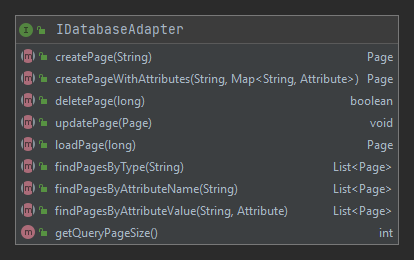
\includegraphics[scale=2.5]{bilder/adapterInterface.png}
\caption{Outline Datenbankadapter Interface}
\end{figure}


Das Ziel war es, ein Interface für die Datenbankfunktionen zu definieren, welches jeden Use Case, der definiert wurde, erfüllen konnte. Daher enthält das Interface IDatabaseAdapter Methoden für die CRUD Operationen und verschiedene Query Methoden.
Anschließend wurden Implementationen dieses Interfaces für jeden Ansatz programmiert. Hier ist zu beachten, das der EAV Ansatz für Oracle und PostgreSQL Datenbank fast identisch ist und wiederverwendet werden konnte. Die Klasse im Programm heißt EAV\textunderscore DatabaseAdapter. Die Implementierung unterscheidet nur beim Auslesen von genierten Primärschlüsseln und der SQL Query zum Suchen von Einträgen mit bestimmten Attributwerten zwischen den Datenbanken.
Da sich die Syntax von Queries mit JSON Inhalten in Oracle und PostgreSQL unterscheiden, wurde für beide Datenbanken jeweils eine JSON Implementation geschrieben. Die zugehörigen Klassen heißen JSON\textunderscore Oracle\textunderscore DatabaseAdapter und JSON\textunderscore Postgres\textunderscore DatabaseAdapter.

Das Package connection enthält alle Klassen, die die Verbindung zu den Datenbanken verwalten. Auch hier gibt es eine Klasse, AbstractConnectionManager, die den Grundaufbau dieser Klassen enthält. Alle Tests wurden nur mit einer einzigen Connection zu der jeweiligen Datenbank durchgeführt, d.h. es finden keine parallelen Zugriffe statt.
Oracle Database und PostgreSQL verwalten mehrere Datenbanken auf einer Instanz unterschiedlich. In Oracle Database lassen sich mehrere Datenbanken am einfachsten mit mehreren Usern umsetzen. PostgreSQL kann stattdessen mehrere Datenbanken mit nur einem Benutzer anlegen. Ein weiterer Unterschied ist der Connection-String bzw. die URL der Datenbank. Diese beiden Besonderheiten werden von den jeweiligen Implementationen beachtet.
Es existiert zusätzlich ein Connection-Manager für eine H2 Datenbank. H2 Database Engine ist eine In-Memory Datenbank, die oft zum Testen von Software und deren Datenbankschnittstellen verwendet wird. Auch in diesem Projekt wurde H2 verwendet, um die Umsetzung des EAV Ansatzes, der komplexe Logik enthält, zu testen. Diese Tests haben den Vorteil, dass sie ohne eine existierende Datenbank durchgeführt werden können. Dies war besonders zum Anfang der Entwicklung, bevor fest beschlossen war, wie die Datenbanken verwaltet werden, sehr hilfreich. Da die JSON Ansätze immer spezielle Syntax für die jeweilige Datenbank besitzen lohnte es sich nicht, Unit-Tests mit H2 für sie zu schreiben. Stattdessen existieren zusätzlich Integrations-Tests für jede Ansatz-Datenbank Kombination. Die Performance Tests, mit denen die Messwerte generiert wurden, haben sich aus diesen Integration Tests heraus gebildet und besitzen eine ähnliche Umsetzung. Die Klasse, die für die Perfomancetests verwendet wurde, heißt CommonCaseSetup.

\label{ppar:Serialisierung}
\paragraph{Serialisierung von Objekten}

Für die Verwendung von JSON Datentypen in Datenbanken müssen Objekte serialisiert werden. Dafür wurde das Framework \textit{gson} verwendet \cite{GitHub.05.07.2021}. Es ermöglicht, \ac{POJO}s in JSON umzuwandeln. Die Komplexität des Einsatzes dieses Frameworks steigt mit der Komplexität der Objekte. Da die umgewandelten Objekte ein bestimmtes Format haben sollen, musste ein spezieller Type-Adapter registriert werden. Type-Adapter erlauben es, spezielle selbst konfigurierte Serialisierer und Deserialisierer bei bestimmten Objekten zu verwenden.
Dies ist der verwendete Aufbau der JSON Objekte:

\begin{lstlisting}[language=json,caption={Attribute-JSON}]
[
    {
        "name": "firstAttribute",
        "values": [
            {
                "String": "firstValue"
            }
        ]
    },
    {
        "name": "secondAttribute",
        "values": [
            {
                "String": "Mustermann"
            }
        ]
    },
    {
        "name": "anotherAttribute",
        "values": [
            {
                "String": "Berlin"
            }
        ]
    }
]
\end{lstlisting}

Dieser Aufbau basiert auf mehreren Ansprüchen. Das Root-Element ist ein Array, das alle gewünschten Attribute enthalten kann. Die Objekte in dem Array haben zwei Schlüssel-Wert Paare. Das erste beschreibt den Namen des Attributs. Das zweite hat als Wert ein Array aus einzelnen Schlüssel-Wert Paaren. Hier wurde ein Array gewählt, um in Zukunft das Speichern von mehreren Werten unter einem Attributnamen zu ermöglichen. In der Praxis wurde diese Fähigkeit nicht verwendet oder untersucht. Das gleiche gilt für den Attributtyp, der den Schlüssel in dem Wert-Objekt bildet. Dieser ermöglicht theoretisch, spezielle Logik basierend auf dem Typ des Attributs anzuwenden, etwa Tests auf Datenintegrität bei einem Typ wie Datum. Letztendlich existierten die Enums für verschiedene Typen, doch das Testprogramm machte keine weiteren Unterscheidungen basierend auf diesen. Der Wert für den Typ-Schlüssel ist schließlich der gespeicherte Wert für das Attribut.
%Object Lifecycle - ähnlich wie hibernate

\subsection{Wiederverwendbarkeit und Reproduktion der Anwendung und Tests}

Der Wunsch, die Testumgebung möglichst wiederverwendbar und einfach aufstellbar zu machen, zeigt sich in mehreren Aspekten der Testapplikation.

Zur Organisation der Abhängigkeiten und des Build-Prozesses wurde Maven verwendet. Maven ist neben Gradle und Apache Ant das am häufigsten verwendete Build-Tool in Java Umgebungen \cite{Sulir.2016}. Maven automatisiert den Download und die Einrichtung aller benötigten Frameworks und Treibern. Die Testanwendung benötigte unter anderem Frameworks zur Durchführung von Unit-Tests, Logging von Ergebnissen, Serialisierung von Objekten und der Verwaltung von Docker Containern. Zusätzlich werden auch passende JDBC Treiber für unsere Datenbank verwaltet, d.h. heruntergeladen und registriert. Eine weitere Hilfe ist Maven für einen benutzerdefinierten Build-Process. In der Testanwendung werden die verwendeten Standard-Schritte validate, compile, test, package und verify mit einem pre-integration-test Schritt erweitert, der die benötigten Docker Images mithilfe bereitgestellter Skripts erstellt. Durch diese Anpassungen wurde die Ausführung des Programms an neuen Maschinen erleichtert.

Eine weitere Entscheidung, die durch diese Mentalität geprägt war, ist, alle Testdatenbanken innerhalb von Docker Containern zu betreiben. Docker ist ein Tool zur Virtualisierung von Containern, die virtuellen Maschinen ähneln. Docker hat jedoch den Vorteil, das alle Container den Kernel teilen können und jeweils nur mit den nötigen Bibliotheken und Tools ausgestattet werden. Dadurch werden Speicherplatz und Performance eingespart. 
Sogenannte Dockerfiles ermöglichen es, Images für Container basierend auf existierenden Images zu erstellen. Diese Technologie wird verwendet, um die Datenbanken reproduzierbar zu konfigurieren. Sowohl PostgreSQL als auch Oracle Database stellen Basis-Images zur Verfügung, die beliebig erweitert werden können. 
Für die Performancetests wurden für jede Datenbankanwendung jeweils ein Dockerfile angelegt. Diese fallen sehr einfach aus. Beide Basis-Images stellen einen Ordner, \lstinline|/docker-entrypoint-initdb.d/| bzw. \lstinline|/docker-entrypoint-initdb.d/setup|, für Skripts bereit. Alle sql-Dateien, die sich in diesem Ordner befinden, werden zur Initialisierung des Containers, sobald die Datenbank bereit ist, automatisch ausgeführt. Die Test-Dockerfiles erweitern die Basis-Images der Datenbanken nur mit einem Befehl, der unsere Skripte, die die Befehle zur Erstellung der benötigten Benutzer und Tabellen enthalten, in diesen Ordner kopieren.

Da Oracle Database keine freie Datenbank ist, ist der Vorgang zur Erstellung des Basis-Images komplizierter als der des PostgreSQL-Images, welches automatisch von DockerHub bezogen werden kann. Stattdessen muss das Image per Hand mit einem Skript, verfügbar unter \url{https://github.com/oracle/docker-images/blob/main/OracleDatabase/SingleInstance/README.md}, gebaut werden. Bei diesem Schritt werden in der Regel die Binaries der Datenbank benötigt. Das ist bei der verwendeten Version (XE) nicht der Fall, da dies die einzige frei verfügbare ist. Daher befinden sich im Projektarchiv der Testanwendung auch alle benötigten Dateien, um die benötigte Version automatisch und ohne Download des oben verlinkten Archivs zu bauen. Da dies ein sehr zeitintensiver Vorgang ist, testet das Skript zunächst, ob auf der Maschine bereits das fertige Image existiert. Falls nicht, wird lokal das Image mithilfe dieser Dateien gebaut. Dieses Verfahren hat den Nachteil, das eventuelle Änderungen von Oracle an dem Image bzw. dem Dockerfile des Images nicht automatisch übernommen werden können.
So können alle benötigten Images automatisch während des Build-Prozesses von maven erstellt werden.
Starten und Stoppen von Containern basierend auf diesen Images wurde mithilfe des Framework Testcontainers erledigt \cite{testcontainers.13.07.2021}. Dieses kann automatisch neue und existierende Container starten und stoppen und stellt die ansonsten dynamischen Ports mithilfe einer statischen Funktion für die Datenbank-Verbindung zur Verfügung.

Wie bereits in der Einleitung beschrieben ist das Testprogramms auf GitHub unter \url{https://github.com/matthias-epos/dynamic-datamodels} verfügbar. Das Projekt sollte sowohl unter Windows als auch Linux Umgebungen ausführbar sein. Nach dem Download des Repositories kann es mithilfe von mvn integration-tests gebaut und getestet werden. Hier muss beachtet werden, dass von jedem Datenbanksystem maximal eine Instanz laufen soll, da es ansonsten zu Fehlern kommen kann. Die Performance Tests wurden durch Aufruf der Klassen innerhalb einer IDE ausgeführt. Diese sind auch per Kommandozeilen Befehl erreichbar. Um Neu-Initialisiergungen der Datenbank und der Testdaten, die besonders bei dem Testfall mit 1.000.000 Einträgen sehr lange dauert, zu vermeiden, muss in dem Benutzer-Ordner ein Testcontainers-Properties-File mit Name \lstinline|.testcontainers.properties| und der Zeile \lstinline|testcontainers.reuse.enable=true| angelegt werden. Dadurch prüft das verwendete Framework zur Verwaltung der laufenden Container, ob bereits eine laufende Instanz existiert und löscht diese nicht mehr am Ende des Tests.


% Maven den Austausch des Programmierteils des Projekts vereinfacht, hilft Docker bei der Verwaltung der Datenbanken. Existierende Images und Skripte zur Erstellung dieser Images, die die Datenbank enthalten, ist dank öffentlicher Ressourcen einfach zu erstellen. PostgreSQL bietet auf DockerHub ein existierendes Image der neusten Version der Datenbank. Dieses lässt sich innerhalb eines Dockerfiles las Basis eines neuen Images referenzieren. In dem Dockerfile wird zusätzlich mehrere Skripte, die für die Erstellung des Datenmodells und der Initialisierung der Testdaten zuständig sind, in das Verzeichnis /docker-entrypoint-initdb.d/ kopiert. Alle .sql Dateien in diesem Ordner werden beim Start des Images automatisch in nach Namen sortierter Reihenfolge ausgeführt.
%Die selbe Funktionalität existiert bei dem Docker Image der Oracle Datenbank. Duch die Lizenzbestimmungen ist es jedoch nicht genauso einfach wie in der PostgreSQL Umgebung das Basis-Image zu bekommen. Oracle bietet mehrere Skripte an, die beim Bauen des Basisimages helfen. Proprietäre Versionen benötigen eine Binärversion der zu verwendeten Datenbank. Nur die Express Edition Versionen können auch ohne diese erstellt werden. Trotzdem wird kein fertiges Image bereitgestellt, sonder es muss selbst gebaut werden. Da dies ein sehr zeitintensiver Vorgang ist, wurde zunächst getestet, ob auf der Maschine bereits das fertige Image existiert. Falls nicht wird lokal das Image mithilfe von Dockerfile des offizielen Repositories von Oracle gebaut. Dieses Verfahren hat den Nachteil, das eventuelle Änderungen von Oracle an dem Image bzw. dem Dockerfile des Images nicht automatisch übernommen werden können.
%Starten und Stoppen von Containern basierend auf diesen Images wurde mithilfe des Testcontainers Frameworks erledigt. Dieses kann automatisch neue und existierende Container starten und stoppen und stellt die ansonsten dynamischen Ports mithilfe einer statischen Funktion für die Datenbank-Verbinder zur Verfügung.

\subsection{Daten}

Für eine möglichst genaue Simulation einer echten Anwendung wären realistische Daten ein großer Vorteil. Es erspart den Notwendigkeit, einen Algorithmus zu schreiben, der passende Daten generiert. Außerdem hat die Art der gespeicherten Daten einen Einfluss auf die Performance der Datenbank. Ohne bekannte Metriken kann nur geschätzt werden, wie viele Einträge existieren, wie viele Attribute sie jeweils haben und wie groß die gespeicherten Attributwerte sind. Es ist jedoch selbst wenn echte Daten existieren meist nicht möglich sie für Forschungsarbeiten zu benutzten, wenn die gesamte Arbeit nicht unter Verschluss bleibt. Selbst dann muss genau geprüft werden, ob Datenschutzbestimmungen eingehalten werden können. Sobald etwa persönliche Daten enthalten sind, müssen die Benutzer laut Datenschutz-Grundverordnung dem Zweck von Analyse zur Verbesserung zugestimmt haben (vgl. Art. 6 DSVGO). Ein Umweg, die Anonymisierung der Daten, ist auch mit viel Aufwand und Gefahr durch Unachtsamkeit verbunden.

In Anbetracht dieser Tatsachen wurde entscheiden, die Testdaten selbst zu generieren. Da die Daten mehrmals für verschiedene Datenbanken generiert werden mussten, werden die Daten basierend auf einem Seed erstellt. Durch die Wiederverwendung dieses Seeds werden stets die selben Daten erstellt und in den Datenbanken abgelegt. So sind die Versuche leichter nachzustellen und die Performance von verschiedenen Datenbanksystemen vergleichbar.

Der Datenerstellungsalgorithmus nimmt vier Parameter:
\begin{itemize}
\item NUMBER{\_}OF{\_}START{\_}ENTITIES \\
Die Anzahl der Objekte mit dynamischer Anzahl an Attributen, die in der Datenbank abgelegt werden. Verwendet: \textbf{100.000 und 1.000.000}
\item NUMBER{\_}OF{\_}START{\_}ATTRIBUTES \\
Die Anzahl an Attributen, die für die generierten Daten verwendet werden. Es wird davon ausgegangen, dass bestimmte Attribute mehrfach verwendet werden. Daher existiert eine Menge von Attributen, von denen bei Erstellung neuer Objekte zufällig welche ausgewählt werden. Verwendet: \textbf{1000}
\item MEAN{\_}NUMBER{\_}OF{\_}ATTRIBUTES \\
Die durchschnittliche Anzahl an Attributen, die ein Objekt haben wird. Die Verteilung der Anzahl ist normalverteilt. Verwendet: \textbf{100}
\item MAX{\_}NUMBER{\_}OF{\_}ATTRIBUTES \\
Die maximale Anzahl an Attributen, die ein Objekt haben kann. Ein einfaches Limit, um Extremfälle zu vermeiden. Verwendet: \textbf{200}
\end{itemize}

Die erstellten Daten haben bloß einfache Werte. Da bei beiden Ansätzen die Werte auf Textwerte umgewandelt werden wurde entschieden, auch nur Textwerte zu erstellen. Die Werte sind alle komplett zufällige Zeichenketten der Länge 16. 

Zusätzlich zu den komplett zufälligen Attributen wurden auch sogenannte Performance-Attribute erstellt. Diese werden zum Testen der Performance der Queries verwendet. Ein Performance-Attribute hat einen bestimmten Namen, eine Funktion zur Erstellung des Wertes und eine Wahrscheinlichkeit. Der Wahrscheinlichkeitswert beschreibt den Prozentsatz der existierenden Objekte, die dieses Attribut bekommen sollen. Die Werte-Funktion gibt in dem konkreten Testaufbau mit gleicher Wahrscheinlichkeit \lstinline|true| oder \lstinline|false| zurück. Dies ermöglicht den Anwendungsfall ``FindByValue'' zu untersuchen. Ein Performance-Attribut mit den Aufbau \lstinline|("testAttribut", () -> String.valueOf(random.nextBoolean()), 50%))| zum Beispiel fügt der Hälfte aller Objekte ein neues Attribut mit dem Namen \lstinline|"testAttribut"| hinzu. Davon hat eine Hälfte den Wert \lstinline|true| und die Andere \lstinline|false|.
Diese Attribute wurden dann für die Performance Tests verwendet, da genau vorhergesagt werden konnte, wie viele Treffer es jeweils ungefähr geben muss.


%testdaten selbst generiert, (echte daten nicht möglich gewesen, da datenschutz)
%selbst generiert basierend auf identischen seed -> identisch
%nur String werte
%keine hierachische Daten, dh nur simple werte -> keine rekursive aufrufe -> nächste komplexitätsstufe



%umsetzun in java -> 
%verscheidene implementationen via interfaces

%datenbanken in docker, damit tests leichte umsetzbar sind für weitere personen (mvn als buildumgebung, fertige befehle um alles laufen zu lassen)
%open source, verfügbar unter https://github.com/matthias-epos/dynamic-datamodels

%viele einschrnkungen: ...


\subsection{Hardware und Laufumgebung}

Die Tests wurden auf einer Windows-Maschine mit der Version Windows 10 20H2, Build 19042.928 durchgeführt. Es besitzt einen Intel Core i5-8250U CPU mit 1.60GHz und stellt 16GB Arbeitsspeicher zur Verfügung. Die Festplatte ist eine SK hynix SC311 SSD mit eine mit \lstinline|winsat| gemessenen Leistung von 456.44 MB/s Lesen und 437.89 MB/s Schreiben.
Alle Tests wurden 30 mal durchgeführt. Jeder Testdurchlauf begann mit einer Warm-up-Phase, bei der die Aufgaben fünf mal ausgeführt wurden, bevor ein weiterer Durchgang gemessen wurde. Der Warm-up Schritt wurde durchgeführt, da sich zeigte, dass sich nach diesem die gemessenen Zeiten eingependelt haben.

\section{Ergebnisse}

Für den allgemeinen Überblick präsentieren die folgenden Grafiken die durchschnittlichen Laufzeiten der verschiedenen Testaufbauten. Die Ergebnisse werden im nächsten Kapitel genauer analysiert und interpretiert.
% Darstellung von Stichprobenmittelwerten
% Statistische Analyse im nächsten Kapitel

\begin{figure}[H]
\centering
\includestandalone[width=0.7\textwidth]{figures/postgresmillion}
\caption{Ergebnisse PostgreSQL 1.000.000 Einträge}
\end{figure}

\begin{figure}[H]
\centering
\includestandalone[width=0.7\textwidth]{figures/postgresthousands}\\
\caption{Ergebnisse PostgreSQL 100.000 Einträge}
\end{figure}

\begin{figure}[H]
\centering
\includestandalone[width=\textwidth]{figures/oracle}\\
\caption{Ergebnisse Oracle Database 100.000 Einträge}
\end{figure}

\begin{figure}[H]
\centering
\includestandalone[width=\textwidth]{figures/oraclevspostgres}\\
\caption{Vergleich Ergebnisse PostgreSQL und Oracle Database 100.000 Einträge}
\end{figure}

%\begin{tikzpicture}
%	\begin{axis}[
%		width = \textwidth,
%		height = 8cm,
%		major x tick style = transparent,
%		ybar=2*\pgflinewidth,
%       bar width=14pt,
%        ymajorgrids = true,
%        ylabel = {Execution time in ms},
%        symbolic x coords={A,B,C,D},
%        xtick = data,
%        xlabel style={align=center},
%        xlabel = \\A: Json w/o index \qquad \qquad \qquad C: EAV w/o index \\ \qquad \qquad B: Json with index  \qquad \qquad \qquad D: EAV with index, 
%        scaled y ticks = false,
%        enlarge x limits=0.18,
%        ymin=0,
%        legend cell align=left,
%                legend style={
%                at={(1,1.05)},
%                anchor=south east,
%                column sep=1ex
%        }
%	]
%	
%	\addplot[style={pU, fill=pU, mark=none}]
%			coordinates {(A, 94)(B, 71)(C, 77)(D, 78)};
%		
%	\addplot[style={pFA, fill=pFA, mark=none}]
%			coordinates {(A, 58)(B, 96)(C, 355)(D, 323)};
%			
%	\addplot[style={pFV, fill=pFV, mark=none}]
%			coordinates {(A, 65)(B, 131)(C, 354)(D, 238)};
%	\addplot[style={pCBA, fill=pCBA, mark=none}]
%			coordinates {(A, 413)(B, 409)(C, 372)(D, 0)};
%	\addplot[style={pDP, fill=pDP, mark=none}]
%			coordinates {(A, 116)(B, 99)(C, 321)(D, 368)};		%	
%	\legend{Update page, Find by Attribute, Find by value, Change Big Attribute, Delete Page}
%	\end{axis}
%\end{tikzpicture}

\subsection{Statistische Analyse der Ergebnisse}

Bei den vorher gezeigten Testwerten handelt es sich nur um Mittelwerte der Stichproben. Jeder Durchlauf der Test-Suite liefert leicht unterschiedliche Ergebnisse. Diese Eigenschaft ist inhärent von Computern und kann nicht umgangen werden. Um die Ergebnisse auch empirisch zu belegen, muss eine Aussage über die Gesamtgrundmengen, d.h. eine imaginäre Menge unendlich vieler Testdurchgänge, erstellt werden. Dafür kann der Welch-Test für mehrere Ansätze und deren Performance-Ergebnisse angewendet werden. Der Welch-Test ist eine Unterkategorie der t-Tests, eine Reihe von Hypothesentests, mit denen ein Mittelwertvergleich von verschiedenen Gesamtmengen, von denen nur eine Teilmenge bekannt ist, durchgeführt werden kann.

Die Nullhypothese des t-Tests ist, dass beide Teilmengen aus derselben Grundmenge entnommen sind. Dies würde für unsere Untersuchung bedeuten, dass unterschiedliche Ansätze keinen Einfluss auf die Performance unserer Testfälle haben. Da wir den Mittelwert zweier verschiedener Mengen vergleichen wollen, würde der Zweistichproben-t-Test verwendet werden. Da die Varianz der Stichproben nicht identisch ist, müsste der Welch-Test angewendet werden. Andere Varianten ermöglichen den Vergleich von einander anhängigen Paaren oder die Abweichung eines bekannten Erwartungswertes gegenüber dem Mittelwert einer Stichprobe. Weitere Voraussetzungen für die Verwendung des t-Tests ist, dass
\begin{itemize}
\item die Standardabweichung der Grundgesamtmenge nicht bekannt ist,
\item die Stichprobe zufällig entnommen und
\item die Grundgesamtheit der Daten normal verteilt ist; oder basierend auf dem zentralem Grenzwertsatz eine Mindestmenge an Proben existiert.
\end{itemize}

Die Normalverteilung unserer Testwerte kann mithilfe des Shapiro-Wilk-Test bewiesen werden. Die Nullhypothese \textbf{$H_{0}$} dieses Tests nimmt an, dass die Grundmenge, d.h. die Laufzeit unendlicher Testdurchgänge, normalverteilt ist. Die Alternativhypothese \textbf{$H_{1}$} ist, dass keine Normalverteilung vorliegt. Der Test kann nicht dazu verwendet werden, einzuschätzen, in welcher Art die Daten von der Normalverteilung abweichen. \cite{Hedderich.2020}

\begin{table}[h]
\caption{P-Werte des Shapiro-Wilsk-Test für alle Test-Szenarien(gerundet auf 3 signifikante Stellen)}
\centering
\resizebox{\columnwidth}{!}{
\begin{tabular}{c|rrrrrr}
\hline \hline
Ansatz & UpdatePage & FindByAttribute & FindByValue & ChangeBigAttribute & DeletePage & CreatePage \\ [0.5ex]
\hline
Postgres-JSON-mit Index-1m & 0,00212 & 0,003 & \textbf{0,17} & 1,38e-05 & 2,06e-07 & 5,64e-07 \\
Postgres-JSON-ohne Index-1m & 0,00041 & 0,0118 & 0,0363 & \textbf{0,0605} & 7,82e-09 & 0,00154 \\

Postgres-EAV-mit Index-1m & 0,000515 & 1,46e-05 & 0,00717 & - & 6,13e-09 & 0,000144 \\
Postgres-EAV-ohne Index-1m & \textbf{0,255} & 0,0214 & \textbf{0,152} & 0,0324 & 5,18e-07 & 3,09e-05 \\

Postgres-JSON-mit Index-100t & 6,55e-09 & 0,00161 & 0,000327 & 1,6e-05 & 2,19e-06 & 4,24e-06 \\
Postgres-JSON-ohne Index-100t & 8,05e-08 & 0,00917 & \textbf{0,454} & 0,00355 & 0,000256 & 7,44e-11 \\

Postgres-EAV-mit Index-100t & 0,00341 & 0,000383 & 5,16e-07 & - & 0,000216 & 6,01e-06 \\
Postgres-EAV-ohne Index-100t & \textbf{0,195} & 0,00797 & 0,000779 & \textbf{0,81} & 0,00147 & 4,48e-07 \\

Oracle-JSON-mit Index-1m & 3,08e-07 & 0,0412 & 1,11e-06 & 2,21e-09 & 1,16e-06 & 2,02e-05 \\
Oracle-JSON-ohne Index-100t & 9,86e-10 & 0,054 & 0,000174 & 1,35e-09 & 9,89e-06 & 3,43e-07 \\
Oracle-EAV-ohne Index-100t & 0,0134 & \textbf{0,139} & 0,000445 & \textbf{0,864} & 1,29e-06 & 4,59e-08
\end{tabular}
}
\label{tab:shapiro}
\end{table}

Tabelle \ref{tab:shapiro} listet die p-Werte des Shapiro-Wilsk Tests für alle Testdimensionen auf. Der p-Wert gibt an, mit welcher Wahrscheinlichkeit die Nullhypothese nicht abgelehnt wird. Sobald dieser Wert unter das Signifikanzniveau $\alpha$ fällt, wird die Nullhypothese abgelehnt. Die Tabelle markiert alle Einträge, in denen der p-Wert kleiner als \(\alpha = 5\%\) ist.
Die Auswertung des Tests zeigt, dass die Testwerte nur sehr spärlich normalverteilt sind. So können bei allen Use-Cases im Testfall PostgreSQL Datenbank Ansatz Json mit Index und 100.000 Einträgen mit 95\% Konfidenz \textbf{$H_{0}$} abgelehnt werden. Stattdessen wird \textbf{$H_{1}$} angenommen, dass die Daten nicht normalverteilt sind. Alle Ergebnisse, die laut der eben verwendeten Punkte normalverteilt sind, sind in Tabelle \ref{tab:shapiro} fett markiert.
Das deckt sich mit der Beobachtung von Tianshi Chen et al.\cite{Chen.2015}. Ähnlich Ihrer Beobachtungen sind die Performancewerte nicht normalverteilt sondern haben vermehrt Ausreißer nach rechts, d.h. die Laufzeit ist besonders groß. Dies ist auch erkennbar an den Boxplots der Testdaten, die im Anschluss näher betrachtet werden, die hauptsächlich nur Ausreißer nach oben verzeichnen.

Dieses Verhalten ist erklärbar. Computer haben eine Mindestlaufzeit für bestimmte Operationen, die jedoch leicht durch unterschiedliche Ereignisse verzögert werden können. Das ist besonders bei dem Testsystem der Fall, bei dem im Hintergrund andere Programme durch Events oder ständigen Aufgaben Rechenleistung in Anspruch nehmen. Aber auch die Datenbanksysteme haben Routinen, die im Hintergrund ausgelöst werden können und selbst CPU-Performance Tests zeigen ähnliche Verhalten. Tianshin Chen et al.\cite{Chen.2015} untersuchten auch die nötige Anzahl an Testdaten, um basierend auf dem Zentralem Grenzwertsatz Normalverteilung anzunehmen. Das Ergebnis war, dass mehrere hundert Testdurchläufe durchgeführt werden müssten. Daher kann auch die Alternative der Voraussetzung von Normalverteilung, eine gewisse Menge an Testdaten, nicht eingesetzt werden.

Da basierend auf diesen Beobachtungen der t-Test nicht bzw. nur mithilfe von Vorbereitung der Daten angewendet werden kann, muss ein Alternativtest angewendet werden. Hier eignet sich der Mann-Whitney-U-Test\footnote{Auch bekannt als Wilcoxon-Mann-Whitney-Test} \cite{Bridge.1999}. Dies ist ein Rang-Analyse Test und wird meistens dann verwendet, wenn die Voraussetzungen für den t-Test nicht gegeben sind. Alle p-Werte des Mann-Whitney-U-Test, die in den folgenden Tabellen aufgelistet sind, wurden auf 3 signifikante Stellen gerundet.

\subsubsection*{Betrachtung des Einfluss des Index}

%\todo[inline]{Signifikanz nur ausreisser, nur einmal vorrechnen, konstant da immer gleiche anzahl testwerte}

Zunächst betrachten wir die Unterschiede zwischen indizierten und nicht indizierten Ansätzen. Da bei dem EAV Ansatz in der Oracle Umgebung keine Indizes erstellt werden konnten überspringen wir in den Vergleich in diesem Aufbau. Außerdem wird auch der Anwendungsfall ``CreatePage'' in den Boxplots nicht betrachtet, da die Performance bei allen untersuchten Variationen fast identisch ist und so schnell ist, dass Unterschiede ignoriert werden können.

\paragraph*{PostgreSQL EAV 100.000 Elemente}
Bei einer Gesamtzahl von 100.000 Elementen sieht der Vergleich bei dem Ansatz EAV wie folgt aus:

%\begin{figure}[htbp]
	%\begin{adjustbox}{max width=1.4\linewidth,center}
%	\centering
%	\begin{subfigure}[b]{0.2\textwidth}
%	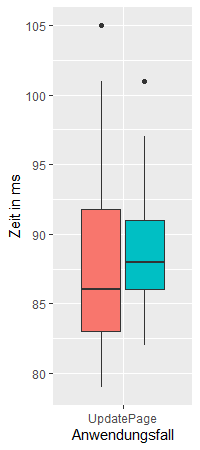
\includegraphics[width=\textwidth]{rStudioPictures/200450.png}

%	\end{subfigure}
%	\rulesep
	%~~~~~~~~
%	\begin{subfigure}[b]{0.7\textwidth}
%		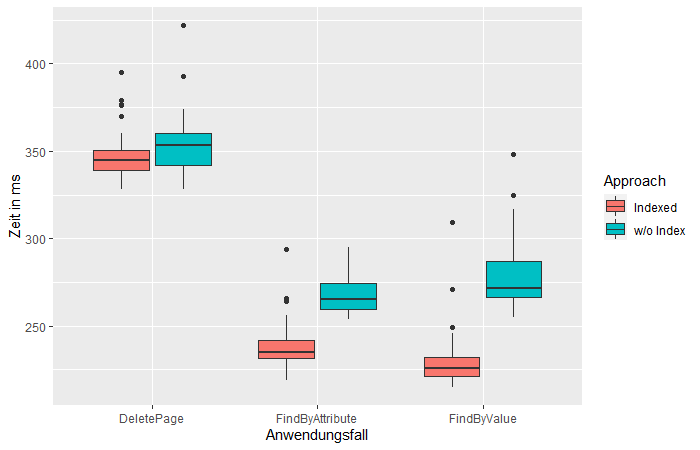
\includegraphics[width=\textwidth]{rStudioPictures/700450.png}
%	\end{subfigure}
	%\end{adjustbox}
%	\caption{Vergleich Performance des Index}
%	\label{fig:postgresEav100kIndex}
%\end{figure}



\begin{figure}[H]
\centering
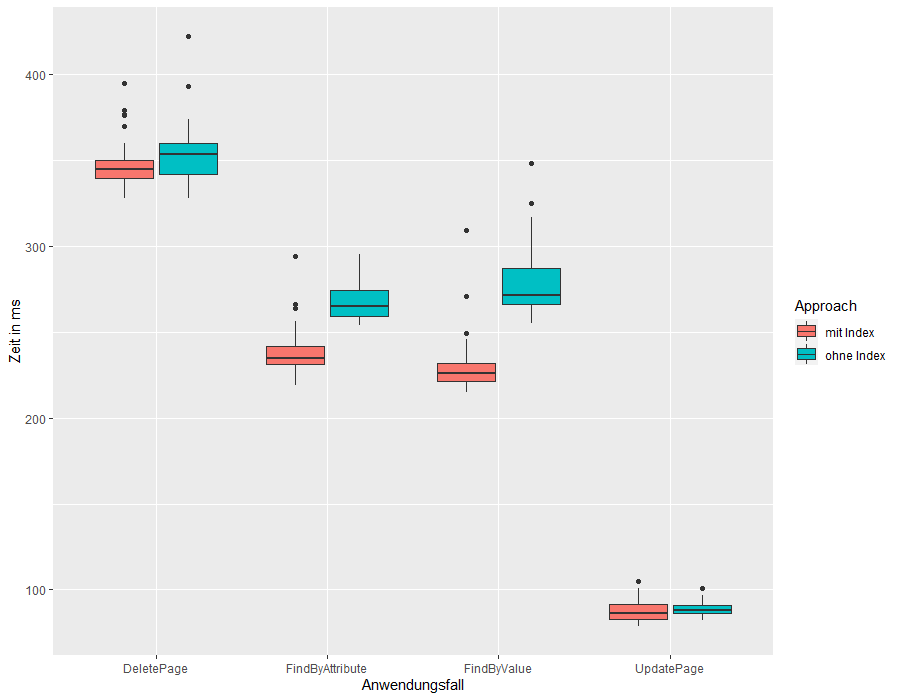
\includegraphics[scale=0.5]{rStudioPictures/postgreseav100kindexfixed900700.png}
\caption{Vergleich Performance mit bzw. ohne Index \\ PostgreSQL, EAV, 100.000 Einträge}
\label{fig:eav100kIndex}
\end{figure}

%Grafik Boxplot EAV 100.000 index vs no index

Hier ist zu beachten, dass der UseCase ``ChangeBigAttribute'' mit einem Index nicht durchgeführt werden konnte, da das zu indizierende Element die maximalen Größe eines Indexeintrags nicht einhalten kann.
%Der Fehler der Datenbank lautet: \todo[inline]{Fehlermeldung nachschauen}.

Unterschiede in der Performance sind vor allem bei den Querys, d.h. den Anwendungsfällen ``FindByAttribute'' und ``FindByValue'', erkennbar. Der Ansatz mit Indizes besitzt anscheinend eine bessere Performance. Ob der Unterschied signifikant ist, kann mithilfe des Mann-Whitney-U-Tests bestimmt werden. Der p-Wert, die für alle Vergleiche in diesem Abschnitt in Tabelle \ref{tab:mwIndexes} aufgelistet sind, gibt Auskunft über die Wahrscheinlichkeit, dass die Nullhypothese korrekt ist. In der Regel wird angenommen, dass ein p-Wert von unter 5\% einen signifikanten Unterschied zwischen den Mengen beweist.
Der p-Wert im Anwendungsfall ''UpdatePage`` liegt bei 0,21. Dieser Wert ist größer als die 5\% Grenze. Daher kann die Nullhypothese nicht abgelehnt werden und es kann kein signifikanter Unterschied festgestellt werden. Dass gleiche gilt für den Anwendungsfall ``DeletePage'', bei dem der Vergleich der Stichproben einen p-Wert von 0,11 ergab. Das deutet an, dass der Index keinen Einfluss auf die Performance bei diesen Anwendungsfällen hat.
Bei den Anwendungsfällen mit Querys hingegen zeigen die Indizes deutlichen und signifikanten Einfluss. Das spiegelt sich auch in den p-Werten: 0,00000000996 für ``FindByAttribute'' und 0,00000000166 für ``FindByValue''. In diesen Fällen ist die Chance, dass die Nullhypothese korrekt ist, verschwindend gering.

In den Beschreibungen der Ergebnisse der meisten folgenden Vergleiche werden die p-Werte nicht explizit aufgelistet. Sie befinden sich jedoch alle am Ende des jeweiligen Abschnitts. Dabei stehen fett markierte Einträge für alle Werte, die sich unter 5\% befinden und daher einen signifikanten Unterschied anzeigen.

\paragraph*{PostgreSQL JSON 100.000 Elemente}
Abbildung \ref{fig:json100kOtherCases} zeigt den Boxplot für den JSON Ansatz mit 100.000 Elementen.

\begin{figure}[H]
\centering
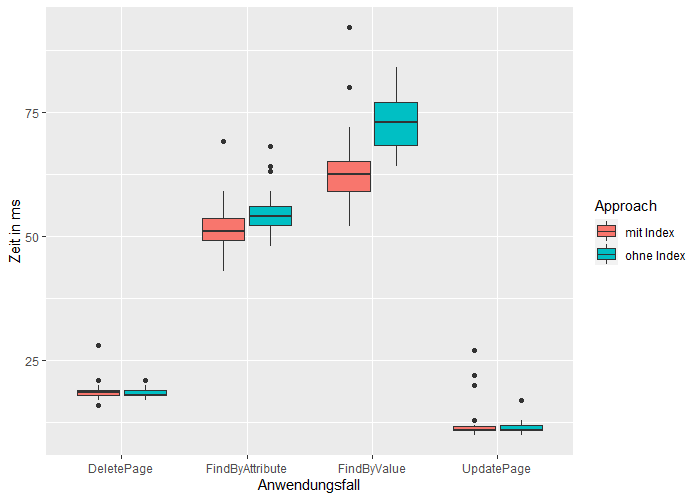
\includegraphics[scale=0.5]{rStudioPictures/json100kIndex700500.png}
\caption{Vergleich Performance mit bzw. ohne Index \\ PostgreSQL, JSON, 100.000 Einträge}
\label{fig:json100kOtherCases}
\end{figure}

Da die Performance des Anwendungsfalls "ChangeBigAttribute" wesentlich langsamer ist, betrachten wir ihn in einer extra Grafik \ref{fig:json100kIndexCBA}.

\begin{figure}[H]
\centering
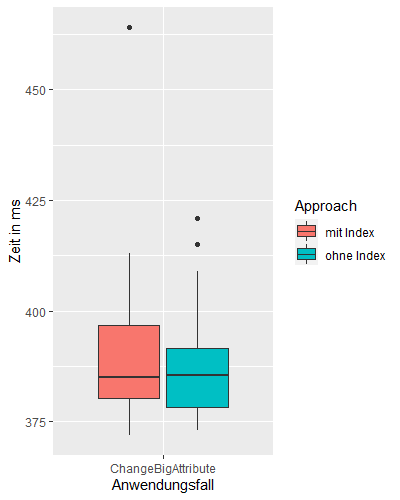
\includegraphics[scale=0.5]{rStudioPictures/json100kIndexCBA400500.png}
\caption{Vergleich Performance mit bzw. ohne Index \\ PostgreSQL, JSON, 100.000 Einträge, Anwendungsfall "ChangeBigAttribute"}
\label{fig:json100kIndexCBA}
\end{figure}

Es zeigt sich ein ähnliches Bild wie bei dem EAV Ansatz. Die Performance der Query-UseCases FindByAttribute und FindByValue profitieren von dem Index, während die anderen UseCases nur geringe Unterschiede haben. Dies belegt auch der Mann-Whitney-U-Test (vgl. Tabelle \ref{tab:mwIndexes}).
% z & r Wert analyse

\paragraph*{PostgreSQL EAV 1.000.000 Elemente}
Um die Performance der Indizes auch für größere Datenmengen einzuschätzen, betrachten wir nun den Vergleich bei einer Million Einträge.

\begin{figure}[H]
\centering
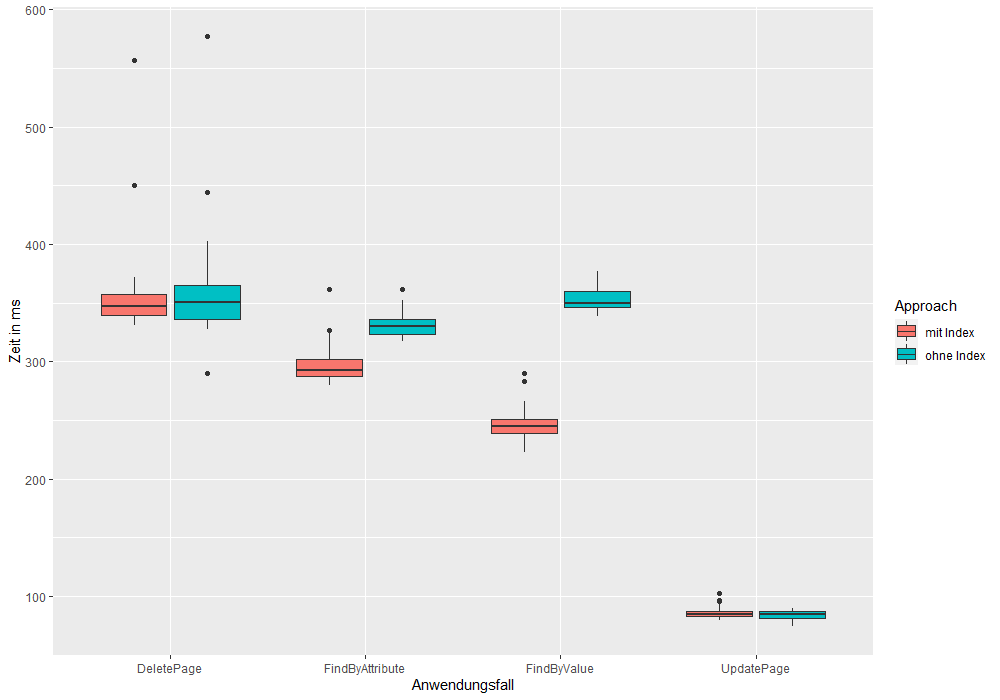
\includegraphics[scale=0.5]{rStudioPictures/eav1mIndexesAll1000700.png}
\caption{Vergleich Performance mit bzw. ohne Index \\ PostgreSQL, EAV, 1.000.000 Einträge}
\label{fig:eav1mIndex}
\end{figure}

Bei dem EAV Ansatz bleibt das Ergebnis ähnlich. Die Querys profitieren und die restlichen Anwendungsfällen verhalten sich fast gleich (vgl. Tabelle \ref{tab:mwIndexes}). Interessanterweise zeigt sich auch ein signifikanter Unterschied der Performance bei der Erstellung von Seiten (in den Boxplots nicht dargestellt). Die Differenz der Medians(mit Index: 4ms, ohne Index: 3ms) von 1ms ist jedoch verglichen mit den anderen Ergebnissen winzig und wird keinen starken Einfluss auf die Gesamtperformance eines Programms haben.


\paragraph*{PostgreSQL JSON 1.000.000 Elemente}
Interessanter ist die Betrachtung des JSON Ansatzes. 

\begin{figure}[H]
\centering
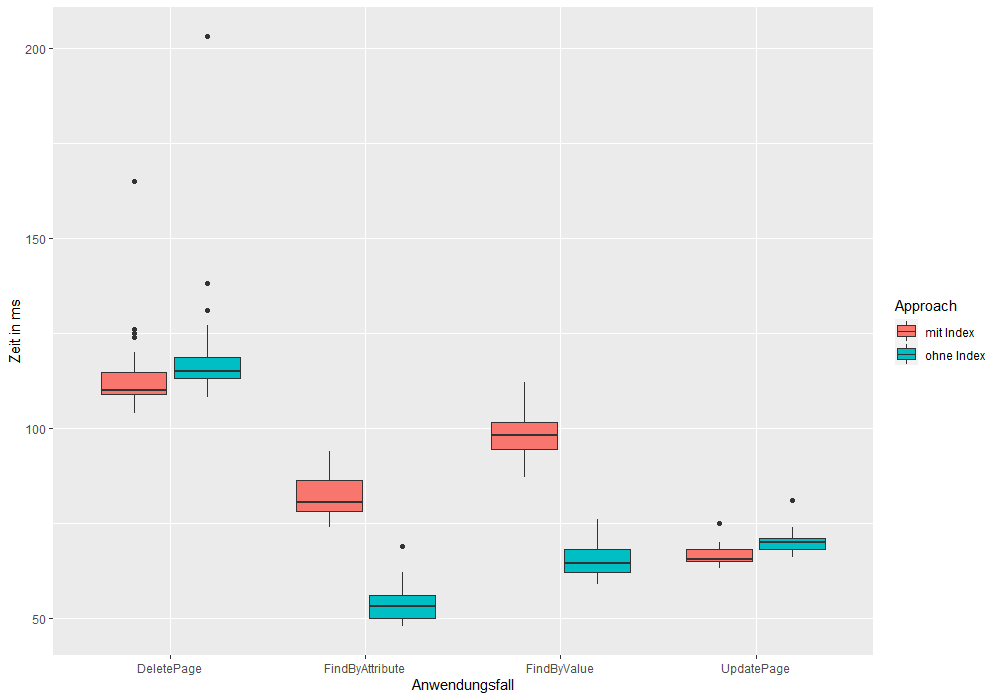
\includegraphics[scale=0.5]{rStudioPictures/json1mIndexes1000700.png}
\caption{Vergleich Performance mit bzw. ohne Index \\ PostgreSQL, JSON, 1.000.000 Einträge}
\label{fig:json1mIndex}
\end{figure}

\begin{figure}[H]
\centering
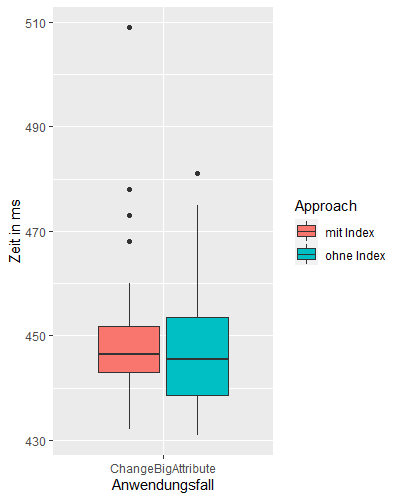
\includegraphics[scale=0.5]{rStudioPictures/json1mIndexesCBA.png}
\caption{Vergleich Performance mit bzw. ohne Index \\ PostgreSQL, JSON, 1.000.000 Einträge, Anwendungsfall "ChangeBigAttribute"}
\label{fig:json1mIndexCBA}
\end{figure}

Der Boxplot hier zeigt das Gegenteil der erwarteten Ergebnisse basierend auf den Bisherigen. Während die anderen Anwendungsfälle weiterhin ähnlich bleiben, ist die Situation bei den Querys invertiert. Die Querys mit Index benötigen wesentlich mehr Zeit zum Abschluss.
Der Anwendungsfall ``ChangeBigAttribute'' ist auf erstem Blick nach wie vor kaum von dem Index betroffen und scheint sich in beiden Fällen ähnlich zu verhalten.
Der zweiseitige Mann-Whitney-U-Test gibt Einblick über den Vergleich der Werte (vgl. Tabelle \ref{tab:mwIndexes}). Die Tests ergeben, dass bei allen Anwendungsfällen bis auf ChangeBigAttribute und CreatePage signifikante Unterschiede existieren. Da laut Boxplot unterschiedliche Ansätze jeweils besser sind betrachten wir in diesem Fall zusätzlich die Alternativhypothesen ``greater'' und ``less''.

\begin{table}[h]
\caption{P-Werte der Alternativhypothesen des Mann-Whitney-U-Tests für den Testaufbau Postgres, 1.000.000 Einträge, JSON; Vergleich mit Index gegenüber ohne Index}
\centering
\resizebox{\columnwidth}{!}{
\begin{tabular}{c|rrrrrr}
\hline \hline
Alternativhypothese & UpdatePage & FindByAttribute & FindByValue & ChangeBigAttribute & DeletePage & CreatePage \\ [0.5ex]
\hline
``less'' & \textbf{6,12e-06} & 1 & 1 & 0,711 & \textbf{0,00197} & 0,747 \\
``greater'' & 1 & \textbf{1,43e-11} & \textbf{1,44e-11} & 0,295 & 0,998 & 0,258 \\

\end{tabular}
}
\label{tab:mw1mAlternative}
\end{table}

Durch unterschiedliche Alternativhypothesen können genauere Aussagen getroffen werden. Während die Hypothese ``two.sided'' nur überprüft, ob ein Unterschied existiert, können die Hypothesen ``less'' und ``greater'' bestimmen, ob die Werte der erste Menge gegnüber der zweiten geringer bzw. größer sind.

\paragraph{Oracle JSON 100.000 Elemente}

Als letztes betrachten wir den Unterschied der Performance in der Oracle Umgebung. Basierend auf den bereits beschriebenen Faktoren, ist in dieser Umgebung nur der Vergleich mit dem Ansatz JSON mit 100.000 Einträgen möglich.

\begin{figure}[H]
\centering
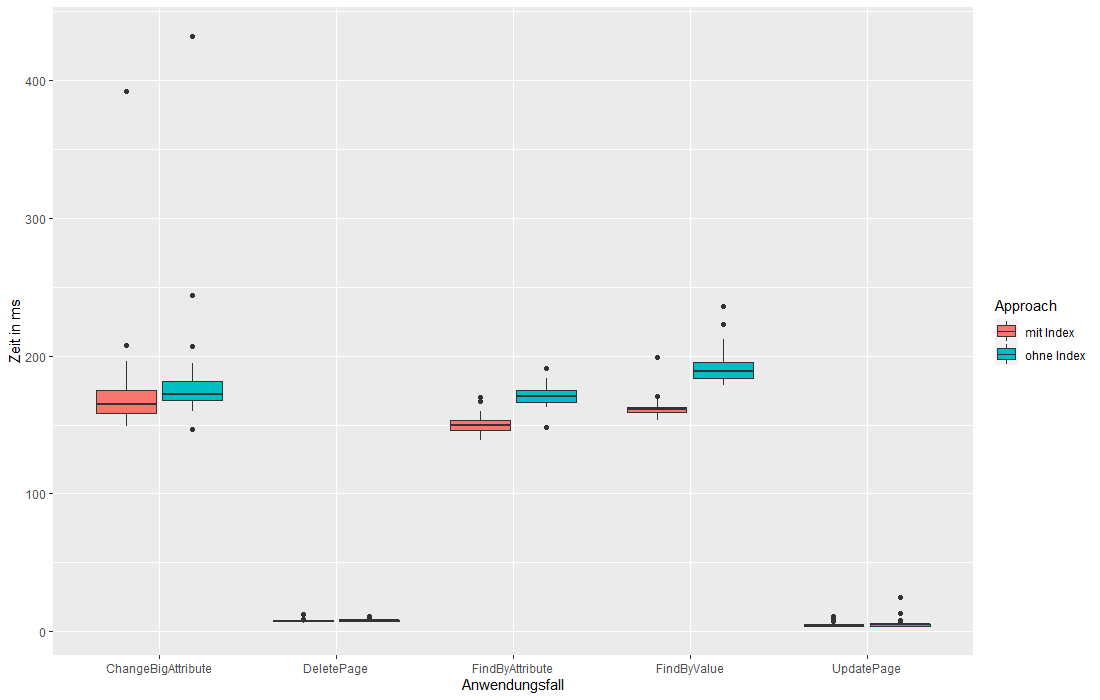
\includegraphics[scale=0.5]{rStudioPictures/oraclejson100kindex1100700.png}
\caption{Vergleich Performance mit bzw. ohne Index \\ Oracle Database, JSON, 100.000 Einträge}
\label{fig:oracle100kIndex}
\end{figure}

Hier ist wieder ein ähnliches Bild wie in den anderen Testkonfigurationen zu sehen. Wie erwartet verbessert der Index die Suche nach bestimmten Einträgen.

Gesamt betrachtet lässt sich sagen, dass sich der Einsatz von Indizes meistens lohnt. Sie haben keinen signifikanten Einfluss auf Update und Delete Zeiten und verbessern meistens die Performance von Querys. Die einzige Ausnahme ist der \ac{GIN} Index bei einer Million Einträgen. Bei diesem Fall verschlechtert sich die Performance signifikant.

\begin{table}[h]
\caption{P-Werte des Mann-Whitney-U-Test mit zweiseitiger Alternativhypothese für den Vergleich zwischen mit und ohne Index(gerundet auf 3 signifikante Stellen)}
\centering
\resizebox{\columnwidth}{!}{
\begin{tabular}{c|rrrrrr}
\hline \hline
Ansatz & UpdatePage & FindByAttribute & FindByValue & ChangeBigAttribute & DeletePage & CreatePage \\ [0.5ex]
\hline
Postgres-EAV-100.000 & 0,218 & \textbf{9,96e-09} & \textbf{1,66e-09} & - & 0,11 & 0,432 \\
Postgres-JSON-100.000 & 0,379 & \textbf{0,0062} & \textbf{5,43e-07} & 0,584 & 0,876 & 0,336 \\
Postgres-EAV-1m & 0,276 & \textbf{3,94e-09} & \textbf{2,96e-11} & - & 0,796 & \textbf{0,00503}\\
Postgres-JSON-1m & \textbf{1,22e-05} & \textbf{2,86e-11} & \textbf{2,87e-11} & 0,589 & \textbf{0,00393} & 0,517\\
Oracle-JSON-100.000 & 0,308 & \textbf{9,34e-10} & \textbf{2,77e-10} & \textbf{0,0308} & \textbf{0,0163} & 0,094
\end{tabular}
}
\label{tab:mwIndexes}
\end{table}

\subsubsection*{Betrachtung des Einfluss des Ansatzes}

Nach dem Vergleich der Performance von Indizes werden nun die Unterschiede zwischen den Ansätzen näher betrachtet. Die Wahl, ob der Aufbau mit oder ohne Indizes verwendet wird, wird auf Basis der vorausgehenden Ergebnisse getroffen. Das bedeutet, dass für den Vergleich bei dem Aufbau mit 100.000 Einträgen die Variationen mit Index verglichen werden. Selbst bei Betrachtung des Aufbaus mit 1.000.000 Einträgen wird nur mit Index verglichen, da die bekannten Unterschiede bei dem JSON Ansatz nicht groß genug sind, um Einfluss auf diesen Vergleich zu haben. Außerdem kann bei dem Anwendungsfall ``ChangeBigAttribute'' und Ansatz EAV nur die Werte ohne Index verwendet werden, da der Test nicht mit Indizes durchgeführt werden konnte.


\paragraph{PostgreSQL 100.000 Einträge}

\begin{figure}[H]
\centering
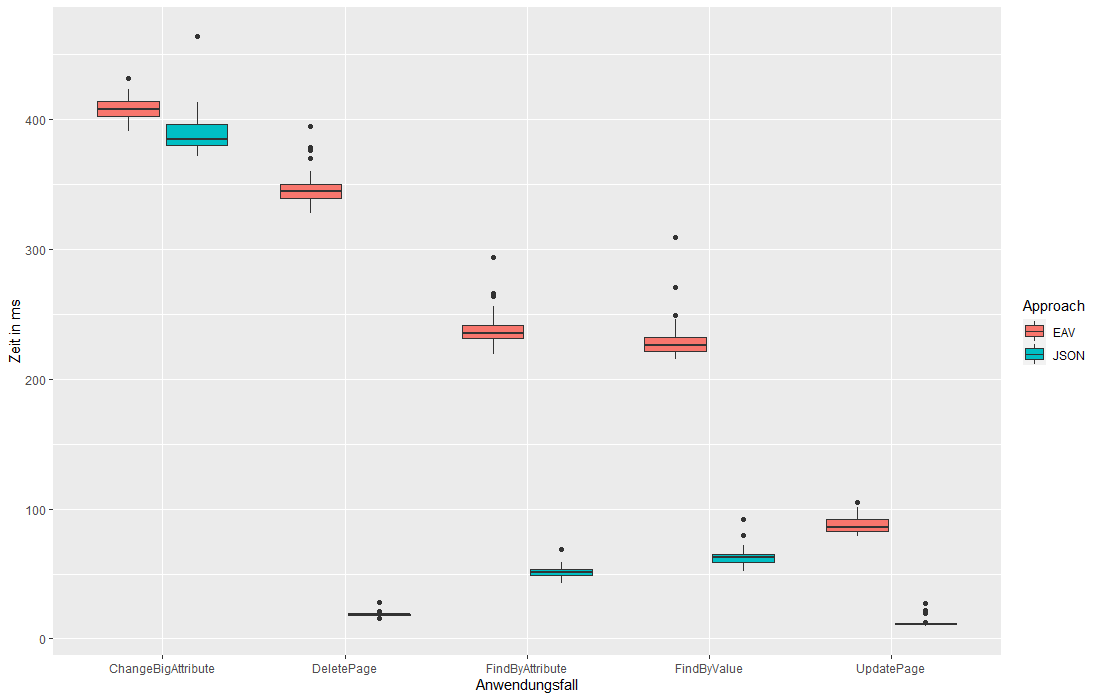
\includegraphics[scale=0.5]{rStudioPictures/postgres100k1100700.png}
\label{fig:ApproachPostgres100k}
\caption{Vergleich Ansätze EAV / JSON \\ PostgreSQL, JSON, 100.000 Einträge}
\end{figure}

Auf ersten Blick ist direkt erkennbar, dass der JSON Ansatz den EAV Ansatz in fast allen Fällen deutlich schlägt. Die einzige Außnahme ist der Anwendungsfall ``ChangeBigAttribute'', der relativ ähnlich lange benötigt. Auch die Ergebnisse des Mann-Whitney-U-Test (vgl. Tabelle \ref{tab:mwApproach}) belegen einen signifikanten Unterschied der Testmengen. Selbst bei dem Anwendungsfall ``ChangeBigAttribute'' gibt es nur eine Chance von 0,00000000156\%, dass die die Nullhypothese korrekt ist und nicht zugunsten der  Alternativhypothese ``two.sided'' abgelehnt wird.


\paragraph{Oracle 100.000 Einträge}
Nach dem Vergleich der Performance bei 100.000 Einträgen bei PostgreSQL wird nun der selbe Vergleich bei Oracle Database betrachtet.

\begin{figure}[H]
\centering
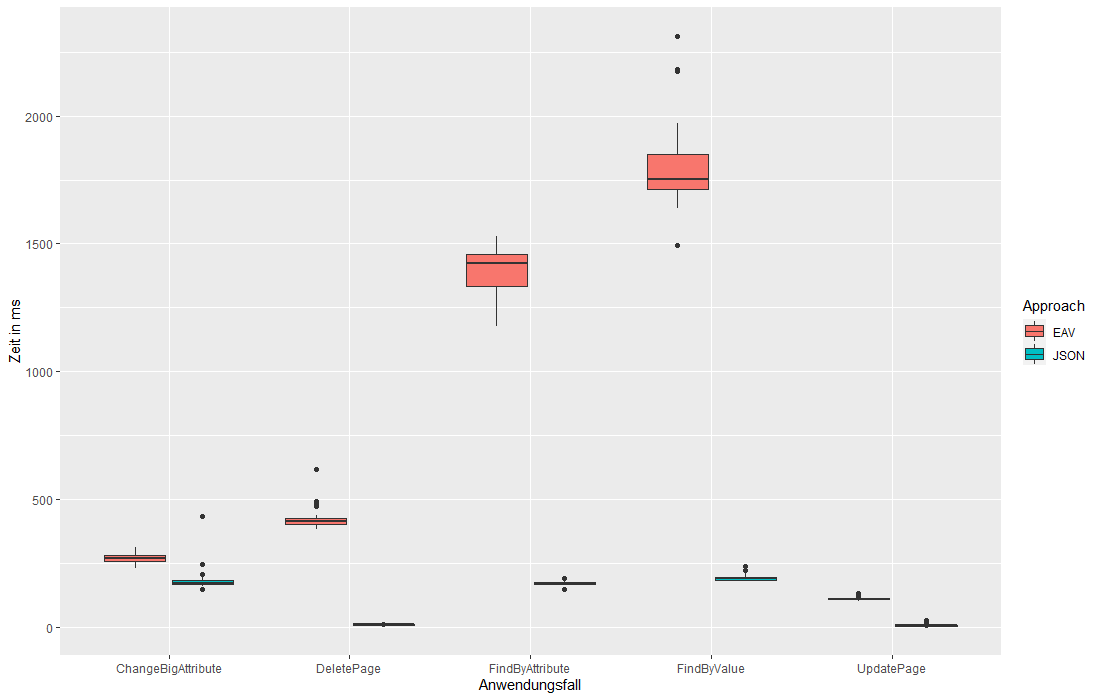
\includegraphics[scale=0.5]{rStudioPictures/oracle100k1100700.png}
\caption{Vergleich Ansätze EAV / JSON \\ Oracle Database, 100.000 Einträge}
\label{fig:ApproachOracle}
\end{figure}

Hier zeigt sich ein ähnliches Bild wie bei dem Vergleich der Ansätze in der PostgreSQL Umgebung. Die benötigte Zeit beim Ansatz EAV für die Querys fallen sogar extremer aus und benötigen länger als der Anwendungsfall ``ChangeBigAttribute'', der bisher immer als langsamster Testfall auffiel. Die Beobachtungen durch den Boxplot werden weiterhin von dem Mann-Whitney-U-Test gedeckt (vgl. Tabelle \ref{tab:mwApproach}).

\paragraph{PostgreSQL 1.000.000 Einträge}

Als letztes werden die Ansätze bei der PostgreSQL Instanz mit 1.000.000 Einträgen verglichen.

\begin{figure}[H]
\centering
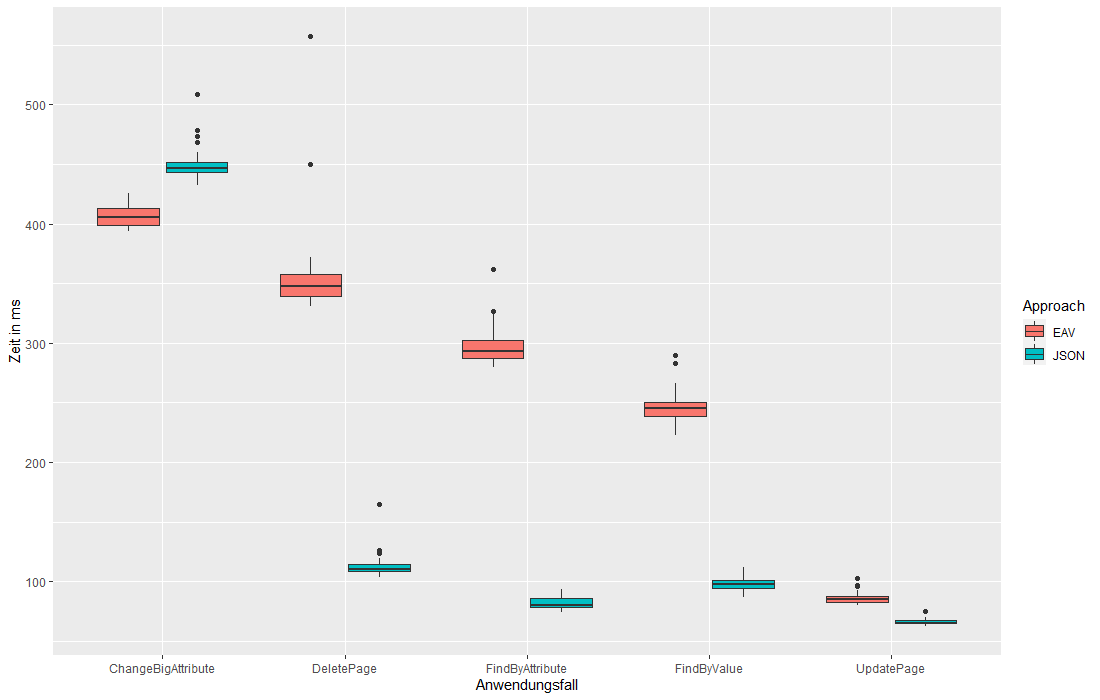
\includegraphics[scale=0.5]{rStudioPictures/postgres1mIndex.png}
\label{fig:ApproachPostgres1m}
\caption{Vergleich Ansätze EAV / JSON \\ PostgreSQL, JSON, 1.000.000 Einträge}
\end{figure}

Hier finden wir die einzige Instanz, in der die JSON Variante langsamer als die zugehörige EAV Variante ist. Das ist bei diesem Vergleich bei dem Anwendungsfall ``ChangeBigAttribute'' der Fall.


\begin{table}[h]
\caption{P-Werte des Mann-Whitney-U-Tests mit Alternativhypothese ``two.sided''; Vergleich der Ansätze EAV und JSON, jeweils mit Index}
\centering
\resizebox{\columnwidth}{!}{
\begin{tabular}{c|rrrrrr}
\hline \hline
Aufbau & UpdatePage & FindByAttribute & FindByValue & ChangeBigAttribute & DeletePage & CreatePage \\ [0.5ex]
\hline
Postgres-100k & \textbf{1,56e-11} & \textbf{2,88e-11} & \textbf{2,93e-11} & \textbf{1,58e-06} & \textbf{2,52e-11} & \textbf{0,0117} \\
Oracle-100k & \textbf{1,95e-11} & \textbf{2,94e-11} & \textbf{2,96e-11} & \textbf{8,05e-10} & \textbf{1,87e-11} & \textbf{0,0445} \\
Postgres-1m & \textbf{2,51e-11} & \textbf{2,93e-11} & \textbf{2,92e-11} & \textbf{2,97e-11} & \textbf{2,85e-11} & \textbf{0,0305}

\end{tabular}
}
\label{tab:mwApproach}
\end{table}

\subsubsection*{Betrachtung des Einfluss des Datenbanksystems}

Zum Abschluss werden die Unterschiede zwischen den Datenbanksystemen betrachtet. Hierfür verwenden wir zuerst die Ergebnisse der Versuche der Datenbankumgebungen mit Indizes und dem JSON Ansatz, da diese eine bessere Performance bei 100.000 Einträgen gezeigt haben.

\begin{figure}[H]
\centering
\includegraphics[scale=0.5]{rStudioPictures/postgresoracle.png}
\caption{Vergleich Datenbankensysteme Oracle Database / PostgreSQL \\ Ansatz JSON, 100.000 Einträge}
\label{fig:DatabasesJSON}
\end{figure}

Während der Werte die Anwendungsfälle ``DeletePage'' und ``UpdatePage'' zwar signifikant unterschiedlich sind, sind die absoluten Zeiten verglichen mit den Anderen Fällen relativ ähnlich, wobei Oracle Database schneller ist. PostgreSQL kann besonders bei den Querys überzeugen. Oracle Database hingegen schlägt sich viel besser bei dem Fall ``ChangeBigAttriubte''.


%Bei der Betrachtung des Boxplots ist sofort die schlechtere Performance von Oracle Database bei den Queries ersichtlich. Eine mögliche Erklärung für die schlechte Performance bei dem UseCase "FindByValue" ist der verwendete Datentyp. Für den Testfall \lstinline|"ChangeBigAttribute|" muss ein Datentyp verwendet werden, der mindestens einen 2MB großen Text speichern kann. Für die Tests wurde daher der Typ clob verwendet. Um innerhalb eines clob Felds nach einem bestimmten Text zu suchen benötigt man eine spezielle Funktion, \lstinline|DBMS_LOB.INSTR()|. Die Verwendung dieser Funktion ist, neben dem Unterschied des Aufrufs von generierten Ids, der einzige Unterschied der Implementierung des EAV Ansatzes für Oracle Database und PostgreSQL. Dieser Unterschied erklärt jedoch nicht den starken Unterschied bei dem Use Case "FindByAttribute", eine Query die auf SQL Ebene identisch umgesetzt ist.

\begin{table}[h]
\caption{P-Werte der Alternativhypothesen des Mann-Whitney-U-Tests für den Vergleich PostgreSQL und Oracle Database, Ansatz JSON}
\centering
\resizebox{\columnwidth}{!}{
\begin{tabular}{c|rrrrrr}
\hline \hline
Alternativhypothese & UpdatePage & FindByAttribute & FindByValue & ChangeBigAttribute & DeletePage & CreatePage \\ [0.5ex]
\hline
``less'' & 1 & \textbf{1,41e-11} & \textbf{1,46e-11} & 1 & 1 & \textbf{2,76e-07} \\
``greater'' & \textbf{1,19e-09} & 1 & 1 & \textbf{2,51e-10} & \textbf{7,89e-12} & 1 \\

\end{tabular}
}
\label{tab:mwDatabasesJSON}
\end{table}

\paragraph{Vergleich EAV Ansatz}

Obwohl sich der EAV Ansatz meistens schlechter schlägt als der JSON Ansatz werden zum Abschluss noch die Ergebnisse der Datenbanken mit EAV verglichen.

\begin{figure}[H]
\centering
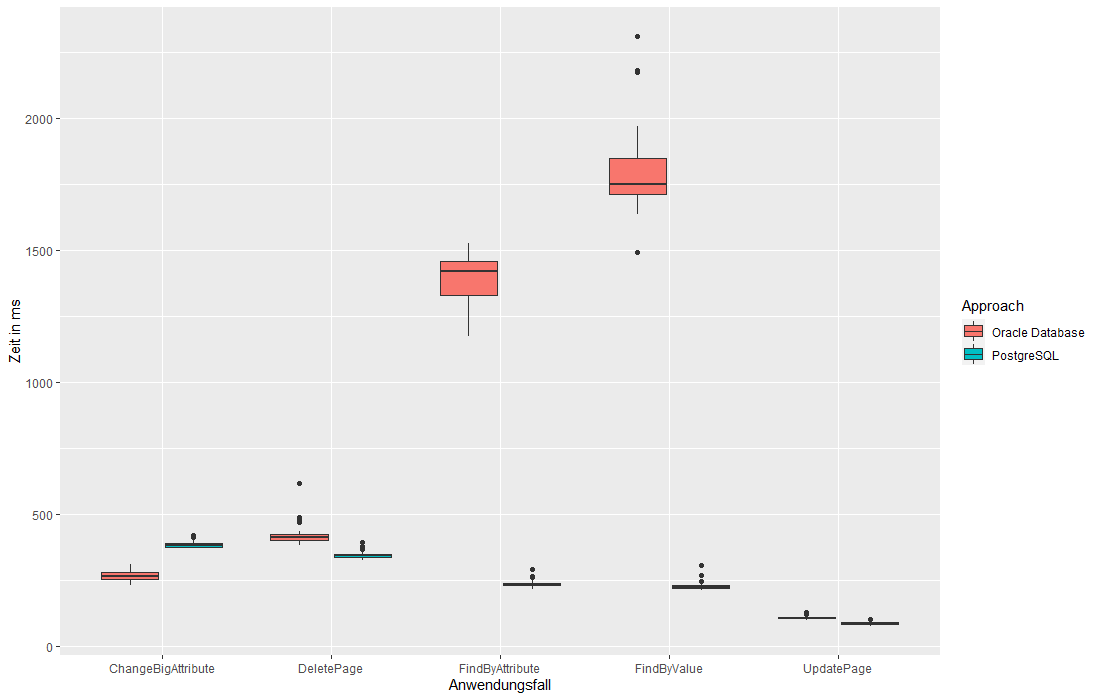
\includegraphics[scale=0.5]{rStudioPictures/oraclepostgreseav100k1100700.png}
\caption{Vergleich Datenbankensysteme Oracle Database / PostgreSQL \\ Ansatz EAV, 100.000 Einträge}
\label{fig:DatabasesEAV}
\end{figure}

Das auffälligste am Vergleich ist die schlechtere Performance von Oracle Database bei den Querries. Hier ist zu beachten, dass bei Oracle Database keine zusätzlichen Indizes eingesetzt werden konnten. Ansonsten ist bemerkenswert, dass die Verhältnisse der Anwendungsfälle ``DeletePage'' und ''UpdatePage'' verglichen mit dem Ansatz JSON invertiert haben.

\begin{table}[h]
\caption{P-Werte der Alternativhypothesen des Mann-Whitney-U-Tests für den Vergleich PostgreSQL und Oracle Database, Ansatz EAV}
\centering
\resizebox{\columnwidth}{!}{
\begin{tabular}{c|rrrrrr}
\hline \hline
Alternativhypothese & UpdatePage & FindByAttribute & FindByValue & ChangeBigAttribute & DeletePage & CreatePage \\ [0.5ex]
\hline
``less'' & \textbf{4,48e-11} & \textbf{1,5e-11} & \textbf{1,49e-11} & 1 & \textbf{2,56e-11} & \textbf{1,57e-06} \\
``greater'' & 1 & 1 & 1 & \textbf{1,49e-11} & 1 & 1 \\

\end{tabular}
}
\label{tab:mwDatabasesEAV}
\end{table}

\subsection{Interpretation der Ergebnisse}

Die statistische Analyse der Ergebnisse hat sowohl erwartete als auch unerwartete Resultate aufgedeckt. Sie beweist auch den Nutzen mehrerer Testdurchläufe. Eine hohe Zahl an Ausreißern nach oben, d.h. Stichproben die untypisch lange dauerten, kann dazu führen, dass Ansätze als gleich bewertet werden. Ein wahrer Performancevergleich kann nur mit genug Stichproben stattfinden. In diesem Abschnitt werden verschiedene Erklärungen und Lösungsvorschläge für Auffälligkeiten in den Ergebnissen in Erwägung gezogen. Sie können als Grundlage für weitere Forschung in Betracht gezogen werden.

\paragraph{Unterschiede Performance PostgreSQL und Oracle Database}

Der Unterschied der Performance zwischen PostgreSQL und Oracle Database mit Ansatz JSON lässt sich leicht kategorisieren. PostgreSQL schlägt Oracle Database bei den Querys, während Oracle bessere Performance bei den restlichen Anwendungsfällen zeigt. Die Erklärung für diese Beobachtung könnte ähnlich wie bei dem CAP-Theorem an den Fokusen der Indizes liegen. Desto schneller Querys basierend auf einem Index sein sollen, desto komplexer ist es, den Index aktuell zu halten. Ein einfacherer Index hingegen kann leichter aktualisiert werden.

Der \ac{GIN} von PostgreSQL ist standardmäßig mit einer ``fast update list'' ausgestattet. In dieser Liste werden Änderungen an den Daten im Index zwischengespeichert, bevor sie mit dem Index zusammengeführt werden. Dies geschieht entweder per Hand oder automatisch, wenn die Liste eine bestimmte Größe überschreitet. Diese Eigenschaft macht es unwahrscheinlicher, dass dies der Grund ist.
Ein anderer Grund könnten die verwendeten Datentypen sein. Während Oracle Database einen Constraint benutzt, besitzt PostgreSQL einen eigenen Datentyp für JSON Felder. Alle Daten, die in einem \lstinline|jsonb| Feld abgelegt werden, werden automatisch in eine Binärrepresentation umgewandelt. Der zusätzliche Aufwand dieser Umwandlung könnte der Einfluss sein, der die Querys erleichtert und die Update Funktion langsamer macht.

Ein weiterer Einfluss auf die Ergebnisse ist das Tuning der Datenbanken. In den Tests wurden die Docker Images der Hersteller benutzt, ohne sie speziell auf die Aufgabenstellung vorzubereiten. Standardeinstellungen, die in diesen Images vorhanden sind, können die Performance auf verschiedene Art und Weise beeinflussen. Außerdem wurden für die Tests die Express Edition von Oracle Database verwendet, die im Gegensatz zu der Enterprise Edition in den Features, etwa der maximalen Größe der Daten, eingeschränkt ist. Auch grundlegende Vergleiche der Performance dieser Datenbanken in anderen Anwendungsfällen werden weiterhin durchgeführt und zeigen Unterschiede in der Performance auf \cite{Martins.2021}.

\paragraph{Schlechte Performance des GIN Index bei vielen Einträgen}

Ein besonders interessantes Ergebnis ist die schlechte Performance des \acf{GIN} der PostgreSQL Datenbank. Eigentlich wird von einem Index erwartet, dass er die Laufzeit von Querys verringert, sobald eine gewisse Menge an Daten vorhanden sind. Die praktischen Tests ergaben jedoch, dass der Index mit steigender Anzahl von Einträgen zu langsameren Querys führte. Während bei 100.000 Einträgen der Anwendungsfall ``FindByValue'' der Testaufbau mit Index beim Vergleich der Mediane etwa 10,5ms schneller ist, fällt die Performance bei einer Millionen Einträgen und ist 33,5ms langsamer als das Gegenstück ohne Index.

Eine erste Annahme für den Grund für diese Performance könnte der Aufbau der Testdaten sein. Indizes für Volltextsuche sind meistens für die Verwendung mit echten Texten optimiert. Unsere Testdaten sind jedoch komplett zufällig generiert. Die Werte der dynamischen Attribute sind eine Folge von 16 zufälligen Zeichen.  Dadurch vermindert sich die Chance, dass sich Werte wiederholen. Die Werte echter Datensätze würden aus einfachen Zahlen und sich wiederholende Wörter oder Zeichenketten bestehen. Die einzigen Werte, die sich in dem Testdatensatz wiederholen, sind die Attributnamen und die Schlüssel. Eine genaue Untersuchung der Funktionsweise des \ac{GIN}, den PostgreSQL in der JSON Umgebung verwendet, hilft bei der Einschätzung dieser Annahme. Bei der Erstellung des Indizes gibt es die Wahl zwischen zwei Klassen von \ac{GIN}, eine Standardversion und die Version \lstinline|jsonb_path_ops|. Hier ist zu beachten, dass der  \lstinline|jsonb_path_ops| Index nur den Operator \lstinline|@>| unterstützt. Der Unterschied liegt in der Art und Weise, wie der Pfad der Elemente in der JSON Struktur in dem Index abgelegt werden. Die Dokumentation des Index benutzt folgendes Beispiel \cite{PostgreSQLDocumentation.2021}: Das JSON-Objekt \lstinline|{"foo": {"bar": "baz"}}| würde bei dem \lstinline|jsonb_path_ops| GIN Index zu einem einzelnen Eintrag führen, der aus einem Hash der Pfadelemente und dem Wert selbst besteht. Die andere Variante erstellt einen Eintrag für jeden Schlüssel auf dem Weg und einen extra für den Wert. Eine Suche für genau dieses Element würde dann einen Eintrag suchen, der alle drei Elemente enthält.
Ein kurzer Test vor den gesamten Testläufen, die in dieser Arbeit besprochen werden, konnte die Angabe der Dokumentation, dass der \ac{GIN} mit der Klasse \lstinline|jsonb_path_ops| schneller ist, nachweisen. Das deckt sich auch mit den Angaben einer Präsentation von Cristophe Pettus von 2015 \cite{PettusChristophe.2015}.
%Aufbau der Daten

Die Dokumentation des \lstinline|jsonb| Dateityps legt auch nahe, dass der Containment Check, d.h. die Operation, die für die Querys benutzt werden, besser für JSON Objekte als für JSON Arrays geeignet ist \cite{PostgreSQLDocumentation.2021}. Leider wird nicht darauf eingegangen, ob diese Eigenschaft auch zu tragen kommt, wenn ein \ac{GIN} verwendet wird. Das Root-Element des JSON Elements, das die Attribute abspeichert, ist ein Array. Die Dokumentation besagt auch, dass Arrays linear durchsucht werden. Da jedoch die durchschnittliche Anzahl an Attributen bei den beiden Test-Setups gleich ist, sollte dies nicht der Grund sein. Selbst falls dies der Fall ist, kann das Array, welches die Attribute beinhaltet, nicht geändert werden, da das gesamte Konzept auf der Fähigkeit der Arrays, eine beliebige Anzahl von Elementen zu enthalten, aufbaut.

Einen weiteren Einfluss auf die Performance des Index haben die Informationen, die dem Querry Builder zur Verfügung stehen. Hier existiert das Problem, das PostgreSQL keine dynamischen Statistiken für Dokumentfelder, darunter der in den Tests verwendete Typ \lstinline|jsonb|, anlegt. Stattdessen wird einfach angenommen, dass der Index 1\% der Reihen trifft \cite{VsevolodSolovyov.08.07.2021, DatabaseAdministratorsStackExchange.08.07.2021}. Dies verfälscht die Wirksamkeit des Index und führt zu schlechten Entscheidungen des Query Planers. 


%schlechte statistiekn


%EVtl da testdaten komplett zufällig -> mit vielen einträgen sehr komplexer index, siehe wie der funktioniernt.

\paragraph{Schlechte Performance des Ansatz EAV bei dem Anwendungsfall ``DeletePage''}

%Bemerkenswert ist, dass das Löschen von Elementen von allen Anwendungsfällen am längsten dauert.  Die durch alle Testvariationen schlechte Performance des Anwendungsfalls ``DeletePage'' mit dem Ansatz EAV kann durch

Bereits bei dem ersten untersuchten Vergleich, PostgreSQL EAV 100.000 Einträge mit und ohne Index, fällt die äußerst schlechte Performance beim Löschen von Elementen. Dieser Vorgang dauert sogar länger als die Suche nach Elementen. Diese Eigenschaft zieht sich durch alle Test-Variationen mit dem Ansatz EAV. Sie kann durch die primitive Umsetzung dieser Methode erklärt werden. Jeder Attributwert nimmt eine Zeile in der Tabelle AttributValues ein. Beim Löschen eines Elements aus der Datenbank wird über die Attribute dieses Elements iteriert und jeder Eintrag in einem eignen SQL-Befehl gelöscht. Ein einziger SQL-Befehl, der alle Einträge mit der Id des zu löschenden Elements entfernt, könnte bereits zu einer Leistungssteigerung führen. 


% OracleJson vs PostgresJSON

% Niedrigste Median per UseCase


\section{Fazit}

Die Programmierung der Testumgebung und das Auswerten der Ergebnisse hat viele interessante Erfahrungen ermöglicht.
Zwar konnte ein funktionales Programm erstellt werden, mit dem dynamische Attribute abgespeichert werden können, doch ein Teil der Features ist mit der Zeit in den Hintergrund gerückt. Dazu gehören die Möglichkeiten, mehrere Werte unter einem Attribut abzuspeichern und eine praktischere Verwendung der Attributtypen. Beide Faktoren sind noch im Design der Anwendung oder des JSON-Elements sichtbar, sind jedoch nicht mit besonderer Logik versehen und könnten mit weiterer Problematiken und Performanceeinbußen verbunden sein. Für den Einsatz in einem realen Programm könnten Stakeholder weitere Features, etwa das Speichern von komplexen Objekten als Attribute oder einer Fuzzy-Suche nach Attributwerten fordern, die das gesamte System noch komplexer machen. Diese Faktoren zeigen zusammen mit den Testergebnissen, warum dies ein Feature mit schlechtem Ruf ist.
Dennoch hat sich bei der Recherche nach bekannten Umsetzungen gezeigt, dass es genug reale Fälle gibt, die genau dieses Feature benötigen, etwa im medizinischen Bereich.

Der Vergleich der Ansätze und die Untersuchung des Einfluss des Datenbanksystems und der Indizes haben mehrere Beobachtungen ermöglicht. 
Der Einsatz von EAV ist mit mehr Programmcode verbunden, ist dadurch fehleranfälliger und hat eine schlechtere Leistung als der JSON Ansatz. Dennoch sollte EAV nicht komplett ignoriert werden. Erstens haben nicht alle Datenbanksysteme so funktionsfähige JSON Unterstützung, wie die beiden die untersucht wurden. Zusätzlich gibt es mehrere Verbesserungspunkte für die Umsetzung. Neben der schlechten Lösch-Performance, die bereits besprochen wurde, könnte der Grundaufbau verbessert werden. Existierende Systeme haben den EAV Ansatz mit einem Klassensystem erweitert. Dies würde den Einsatz speziellere Indizes ermöglichen. Auch die Datenbankfunktion Views, mit denen die Performance häufiger Joins verbessert werden kann, zu erstellen, wurde noch nicht untersucht und könnte den Unterschied in der Performance verbessern.

Der JSON Ansatz im Gegenzug war einfacher umzusetzen. Dies könnte an Erfahrungen mit dieser Datenrepräsentationsart liegen, da JSON auch bei der Programmierung von Webschnittstellen oder in Konfigurationsdateien Einsatz findet. Außerdem wurden in den Tests keine komplexen Objekte verwendet, was die Serialisierung erleichterte. Ein deutlicher Nachteil ist jedoch, dass jede Implementation stark an des verwendete Datenbanksystem gekoppelt ist. Beide Datenbankanbieter, die untersucht wurden, hatten eine eigene Syntax für Querys für Inhalte dieses Typs und spezielle Datentypen. Daher muss bei der Programmierung das Zielsystem bekannt sein. Diese Eigenschaft beeinflusst auch die vorhandene Dokumentation. Desto spezieller ein Feature ist, desto schwieriger ist es, Lösungen für häufige Probleme oder Anleitungen zu finden.
Ein Problem, welches sich bei den Tests zeigte, ist die schlechte Performance des \ac{GIN} der PostgreSQL Datenbank. Recherche für dieses Problem führte zu weiteren Schwächen. Fehlende Statistiken für den Index erschweren richtige Query Planung, was zu schlechterer Performance führt. Hier wäre der Vergleich zu dem Oracle Full-Text-Search Index sehr interessant gewesen, was zu einem weiteren Problem führt.
Das Lizenzmodel der Oracle Datenbank erschwert die Forschung mit dieser. Die Einschränkung, dass die freie Datenbank maximal 12GB groß sein darf, machte die Tests mit mehr Testeinträgen unmöglich und verwehrt die Möglichkeit, die Indizes in genau der Umgebung zu testen, in der ihre Performance besonders wichtig ist.



Generell kann basierend auf den Testergebnissen folgende Entscheidung empfohlen werden:
Falls die verwendete Datenbank einer der beiden untersuchten ist, hat sich der JSON Ansatz in allen Anwendungsfällen als besser erwiesen. Die Wahl zwischen den Datenbanksystemen kann basierend auf der Wichtigkeit oder Menge der Anwendungsfälle getroffen werden. Liegt der Fokus auf Querys, d.h. der Suche nach Elementen mit bestimmen Attributen oder Attributwerten, empfiehlt sich PostgreSQL. Falls jedoch die Dauer von Update und Delete Operationen wichtiger ist, fällt die Wahl eher auf Oracle Database.

Hier werden natürlich viele weitere Faktoren, die die Wahl der Datenbank beeinflussen können, ignoriert. Eine solche Eigenschaft ist die Erst-Einrichtung der Datenbank. In der Docker-Umgebung, in der die Tests durchgeführt wurden, war die Einrichtung der PostgreSQL Datenbank einfacher, da das Basisimage bereits fertig gebaut auf DockerHub verfügbar ist. Andere Faktoren sind z.B. die Kosten, existente Kenntnisse mit den Datenbanken, die Verwaltungstools, Zugriffsverwaltung und viele mehr.

Falls keine der beiden Datenbanken verfügbar ist, ist der EAV Ansatz trotzdem nicht zu unterschätzen. Die Performance ist jedoch viel stärker von der Implementation als von der Datenbank abhängig, da die Verwaltung der Attributwerte in der Datenbank komplexer ist und per Hand programmiert werden muss. Dadurch entstehen mehr Möglichkeiten, Fehler und schlecht performanten Code zu schreiben.

% Ein Feature, das zurecht als problematisch angesehen wird
% Aber ist Teil realler Anwendungsfälle
% Einforderung gewohnter Features macht Umsetzung noch schwerer
% EAV -> Basisversion langsamer als JSON
% JSON, angenehm, da auf bekannter Technologie
% Unterschiedliche Syntax und Datentypen machen ungekoppelte Verwendung schwerer
% Schlechte Statistiken für Index erschweren Optimierung
% Schwache Performance bei vielen Einträgen, sletener Eingestzt, weniger Dokumentation
% Einschränkgunen des Lizenzmodells erschweren Forschung, Vergleich Index mit vielen Einträgen wäre sehr interesant gewessen
% Für eine realle Umsetzung Entscheiden immer JSON, ob Querry oder Update schneller sein sollen + Viele andere Faktoren Oracle doer PostgreSQL (Einrichtung der TEsts einfacher mit Postgres)


